% mnras_template.tex
%
% LaTeX template for creating an MNRAS paper
%
% v3.0 released 14 May 2015
% (version numbers match those of mnras.cls)
%
% Copyright (C) Royal Astronomical Society 2015
% Authors:
% Keith T. Smith (Royal Astronomical Society)

% Change log
%
% v3.0 May 2015
%    Renamed to match the new package name
%    Version number matches mnras.cls
%    A few minor tweaks to wording
% v1.0 September 2013
%    Beta testing only - never publicly released
%    First version: a simple (ish) template for creating an MNRAS paper

%%%%%%%%%%%%%%%%%%%%%%%%%%%%%%%%%%%%%%%%%%%%%%%%%%
% Basic setup. Most papers should leave these options alone.
\documentclass[usenatbib]{mnras}
%\pdfminorversion=5

% MNRAS is set in Times font. If you don't have this installed (most LaTeX
% installations will be fine) or prefer the old Computer Modern fonts, comment
% out the following line
%\usepackage{newtxtext,newtxmath}
% Depending on your LaTeX fonts installation, you might get better results with one of these:
%\usepackage{mathptmx}
%\usepackage{txfonts}

% Use vector fonts, so it zooms properly in on-screen viewing software
% Don't change these lines unless you know what you are doing
\usepackage[T1]{fontenc}
\usepackage{ae,aecompl}
\usepackage{hyperref}
%\usepackage{ulem}

%%%%% AUTHORS - PLACE YOUR OWN PACKAGES HERE %%%%%

% Only include extra packages if you really need them. Common packages are:
\usepackage{graphicx}	% Including figure files
\usepackage{amsmath}	% Advanced maths commands
\usepackage{amssymb}	% Extra maths symbols
\usepackage{multirow}
\usepackage[usenames,dvipsnames,svgnames,table]{xcolor}
\usepackage{verbatim}

%\hypersetup{draft}

%%%%%%%%%%%%%%%%%%%%%%%%%%%%%%%%%%%%%%%%%%%%%%%%%%

%%%%% AUTHORS - PLACE YOUR OWN COMMANDS HERE %%%%%

% Please keep new commands to a minimum, and use \newcommand not \def to avoid
% overwriting existing commands. Example:
%\newcommand{\pcm}{\,cm$^{-2}$}	% per cm-squared

\newcommand{\homsun}{\,h^{-1} {\rm M_\odot}}
\newcommand{\hmsun}{\,h^{-2} {\rm M_\odot}}
\newcommand{\msun}{{\rm M_\odot}}
\newcommand{\hkpc}{\, h^{-1}{\rm{kpc}} }
\newcommand{\hMpc}{\, h^{-1}{\rm{Mpc}} }
\newcommand{\magn}{\, {\rm mag} }

\newcommand{\hsmsun}{\,h_{70}^{-2} {\rm M_\odot}}
\newcommand{\hskpc}{\, h_{70}^{-1}{\rm{kpc}} }
\newcommand{\hsMpc}{\, h_{70}^{-1}{\rm{Mpc}} }
\newcommand{\hsGpc}{\, h_{70}^{-1}{\rm{Gpc}} }

\newcommand{\lan}{\langle}
\newcommand{\ran}{\rangle}

\newcommand{\lcdm}{{\rm \Lambda CDM}}
\newcommand{\am}{\, {\rm arcmin}}
\newcommand{\as}{\, {\rm arcsec}}
\newcommand*{\mean}[1]{\overline{#1}}
\newcommand*{\E}[1]{\times 10^{#1}}
\newcommand{\un}[1]{_{\rm #1}}

\newcommand*{\swap}[2]{#2#1}

%%%%%%%%%%%%%%%%%%%%%%%%%%%%%%%%%%%%%%%%%%%%%%%%%%

%%%%%%%%%%%%%%%%%%% TITLE PAGE %%%%%%%%%%%%%%%%%%%

% Title of the paper, and the short title which is used in the headers.
% Keep the title short and informative.
\title[Extending the RAR with KiDS weak lensing]{Extending the Radial Acceleration Relation using Weak Gravitational Lensing with the Kilo-Degree Survey}
% The list of authors, and the short list which is used in the headers.
% If you need two or more lines of authors, add an extra line using \newauthor
\author[M. M. Brouwer et al.]{Margot M. Brouwer$^{1,2}$\thanks{E-mail:brouwer@astro.rug.nl}, K. A. Oman$^{1,3}$
	 %Group 1:
	 %Group 2:
	 %Group 3:
	\\
	\\
	% List of institutions
	$^{1}$Kapteyn Astronomical Institute, University of Groningen, PO Box 800, NL-9700 AV Groningen, the Netherlands.\\
	$^{2}$Institute for Theoretical Physics, University of Amsterdam, Science Park 904, 1098 XH Amsterdam, The Netherlands. \\
        $^{3}$Institute for Computational Cosmology, Department of Physics, Durham University, South Road, Durham DH1 3LE, UK \\
}

% These dates will be filled out by the publisher
\date{Accepted XXX. Received YYY; in original form ZZZ}

% Enter the current year, for the copyright statements etc.
\pubyear{2019}

% Don't change these lines
\begin{document}
\label{firstpage}
\pagerange{\pageref{firstpage}--\pageref{lastpage}}
\maketitle

% Abstract of the paper
\begin{abstract}
TBW
\end{abstract}


% Select between one and six entries from the list of approved keywords.
% Don't make up new ones.
\begin{keywords}
gravitational lensing: weak -- Surveys -- methods: statistical -- galaxies: haloes -- cosmology: dark matter, theory -- gravitation.
\\
\end{keywords}

%\newpage
\clearpage

%%%%%%%%%%%%%%%%%%%%%%%%%%%%%%%%%%%%%%%%%%%%%%%%%%

%%%%%%%%%%%%%%%%% BODY OF PAPER %%%%%%%%%%%%%%%%%%


\section{Introduction}
\label{sec:introduction}

It has been known for several decades that the outer regions of galaxies rotate faster than would be expected from Newtonian dynamics based on their luminous, or `baryonic', mass. This was first discovered by \cite{rubin1983} through measuring galactic rotation curves of optical disks, and by \cite{bosma1981} through measuring hydrogen profiles at radii beyond the disk. The excess gravity implied by these measurements has been generally attributed to an unknown and invisible substance named Dark Matter (DM), a term coined more than forty years prior by \cite{zwicky1937} when he discovered the so-called `missing mass problem' through the dynamics of galaxies in clusters.

Following more recent observations using Weak gravitational Lensing \cite[WL,][]{hoekstra2004,linden2014,mandelbaum2015}, Baryon Acoustic Oscillations \cite[BAO's,][]{eisenstein2005,blake2011} and the Cosmic Microwave background \cite[CMB,][]{spergel2003,planck2014}, Cold Dark Matter\footnote{DM particles that moved at non-relativistic speeds at the time of recombination, as favoured by measurements of the CBM \cite[]{planck2014} and the Lyman-$\alpha$ forest \cite[]{viel2013}.} (CDM) became a key ingredient of the current standard model of cosmology: the $\lcdm$ model. In this paradigm, CDM accounts for $\Omega_{\rm CDM}=0.266$ of the critical density in the Universe, while baryonic matter only accounts for $\Omega_{\rm CDM}=0.049$ \cite[]{planck2018}. The cosmological constant $\Lambda$, which is necessary to explain the accelerated expansion of the Universe and is usually associated with Dark Energy (DE), accounts for $\Omega_{\rm \Lambda}=0.685$.

Although the $\lcdm$ model successfully describes the behaviour of DM on a wide range of scales, no conclusive evidence for the existence of DM particles has been found so far \cite[despite years of enormous effort; for an overview, see][]{bertone2005,bertone2018}. This still leaves some room for alternative theories of gravity, such as Modified Newtonian Dynamics  \cite[MOND,][]{milgrom1983} and the more recent theory of Emergent Gravity \cite[EG,][]{verlinde2016}. In these theories particle DM does not exist, and all gravity is due to the baryonic matter (or, in the case of EG, the interaction between baryons and the entropy associated with DE). Hence, one of the main properties of these theories is that the mass discrepancy in galaxies correlates strongly with their baryonic mass distribution.

Such a correlation has indeed been widely observed. First astronomers discovered the Tully-Fisher relation \cite[TFR,][]{tully1977} between the luminosity of a spiral galaxy and its asymptotic rotation velocity \cite[]{pierce1988,bernstein1994}. Since this corresponds to a relation between the baryonic and the total galaxy mass, this has later been named the `baryonic' TFR \cite[BTFR,][]{mcgaugh2000,mcgaugh2012}. As the radial resolution of observations increased, astronomers found a strong correlation between the observed rotation velocity $v\un{obs}(r)$ as a function of galaxy radius $r$, and the enclosed luminous mass \mbox{$M\un{b}(<r)$} \cite[]{sanders1986,sanders1996,mcgaugh2004,sanders2007,wu2015}. Since $M\un{b}(<r)$ corresponds to the \emph{expected} gravitational acceleration $g\un{b}(r)$ from baryonic matter, and the observed gravitational acceleration can be calculated through $g\un{obs}(r)=v\un{obs}^2(r)/r$, this relation has been named the Radial Acceleration Relation (RAR)\footnote{Another well-established name for this same relation is the Mass-Discrepency Acceleration Relation (MDAR), which refers to the correspondence between the observed baryonic/total mass and the inferred mass discrepancy commonly attributed to DM. Throughout this work we use the term RAR for brevity.}.

Particularly, the latest results from \cite{mcgaugh2016} (hereafter M16) have measured the RAR relation with unprecedented accuracy, using the Spitzer Photometry and Accurate Rotation Curves \cite[SPARC,][]{lelli2016b} data of 153 late-type galaxies. Their results showed a tight correlation between $g\un{obs}$ and $g\un{bar}$, which they could fit using a simple double power law (Eq. 4 in M16) depending only on $g\un{bar}$ and one free parameter: the acceleration scale $g\un{\dagger}$ where Newtonian gravity appears to break down. This sparked the interest of scientists working on alternative theories of gravity, but also of those in favor of a statistical explanation of the RAR within the $\lcdm$ framework \cite[]{keller2017,desmond2017,ludlow2017}.

The latter possibility was quantified by \cite{navarro2017} (hereafter N17) who used a range of simplifying assumptions based on galaxy observations and DM simulations, in order to create an analytical galaxy+halo model. The goal of their model was to reconstruct the RAR in galaxies, in particular the value of $a\un{0}$: the acceleration scale where the relation transitions from the baryon-dominated to the DM-dominated regime (which is equivalent to $g\un{\dagger}$), and $a\un{min}$: the minimum acceleration probed by galaxy disks. Based on their results, they claimed that the RAR can be explained within the $\lcdm$ framework, at the accelerations probed by galaxy rotation curves (i.e. $g\un{obs}>a\un{min}$). However, since their model relies on the fact that luminous kinematic tracers in galaxies only probe a limited radial range, N17 predicted that extending observations to radii beyond the disk (which correspond to lower gravitational accelerations) would lead to systematic deviations from the simple relation posed by M16.

The goal of this work is to extend observations of the RAR to lower accelerations, which are not measurable using galaxy rotation curves. To this end we use gravitational lensing: the perturbation of light inside a gravitational potential as described by General Relativity (GR). In particular, we use the method of Galaxy-Galaxy Lensing (GGL): the statistical measurement of the coherent image distortion (shear) of a field of background galaxies by the gravitational potential of a sample of foreground galaxies \cite[for examples, see e.g.][]{fischer2000ggl,hoekstra2004,mandelbaum2006,uitert2016}. Using GGL we can measure the average (apparent) density distribution of galaxies up to a radius of $3\,{\rm Mpc}$, roughly a $100$ times larger than the radius of the luminous disk ($\sim 30\,{\rm kpc}$), corresponding to a value of $g\un{bar}$ that is $3$ orders of magnitude lower than those measurable with galaxy rotation curves.

First, we measure the baryonic and total density profiles of our galaxies through their luminosities and GGL profiles. These measurements will be performed using photometric data from Sloan Digital Sky Survey \cite[SDSS,]{abazajian2009} and the VISTA Kilo-Degree Infrared Galaxy survey \cite[VIKING]{edge2013}, and WL data from the Kilo-Degree Survey \cite[KiDS;][]{dejong2013}. We then translate these measurements into the baryonic and observed radial accelerations, $g\un{bar}$ and $g\un{obs}$. Finally, we compare the resulting RAR to predictions from different modified gravity theories (MOND and EG) and $\lcdm$.

The $\lcdm$ predictions will not only be provided by the N17 analytical model, but also by two mock galaxy catalogues based on two different DM simulations. One is the Marenostrum Institut de Ci{\`e}ncies de l'Espai (MICE) Galaxy and Halo Light-cone catalogue \cite[]{carretero2015,hoffmann2015}, which is based on the MICE Grand Challenge lightcone simulation \cite[MICE-GC,][]{fosalba2015a,fosalba2015b,crocce2015}. The other mock galaxy catalogue is based on a suite of large-volume cosmological hydrodynamical simulations, which is called the BAryons and HAloes of MAssive Systems (BAHAMAS) project \cite[]{mccarthy2017}. Our final goal is to distinguish which of the aforementioned predictions best describe the RAR at lower accelerations.

Having almost a million foreground galaxies at our disposal, we are able to select specific galaxy samples designed to optimally test these predictions. Particularly, we note that most models (MOND, EG, and the N17 analytical DM model) focus on the description of individual, isolated galaxies. In order to test them, therefore, we select a sample of galaxies whose lensing profiles are not affected by their neighbours within the radius of our measurement. In contrast, the predictions from the MICE and BAHAMAS simulations can be tested for both isolated and non-isolated galaxy samples.

Furthermore, we note that all models give a specific prediction regarding the dependence of the RAR on baryonic galaxy mass. According to the MOND and EG theories, the relation between $g\un{bar}$ and $g\un{obs}$ should remain intact in the regime beyond the disk, independent of the disk mass. Within the $\lcdm$ paradigm, however, all predictions (analytical and simulated) are based on a `stellar-to-halo-mass relation' which is not constant as a function of baryonic galaxy mass. By splitting our foreground galaxies into bins of increasing stellar mass, we are able to better distinguish the predictions of these different models.

Our paper is structured as follows: In Sect. \ref{sec:data} we introduce our main datasets: both the KiDS and GAMA galaxy surveys which are used to perform the GGL measurements, and the MICE and BAHAMAS simulations \& mock galaxy catalogues to which we compare our results. Sect. \ref{sec:analysis} describes our analysis of these (mock) datasets as we select our isolated foreground galaxy sample, perform the GGL measurements, and translate the results into the RAR. Sect. \ref{sec:theories} contains a description of the theoretical predictions to which we compare our observations: MOND, EG and the N17 analytical DM model. In Sect. \ref{sec:results} we present the resulting RAR measurements and model comparison. Sect. \ref{sec:discon} contains the discussion and conclusion.

Throughout this work we adopt the WMAP 9-year \cite[]{hinshaw2013} cosmological parameters: $\Omega\un{m}=0.2793$, $\Omega\un{b}=0.0463$, $\Omega\un{\Lambda}=0.7207$, $\sigma_8=0.821$ and $H_0 = 70 \, {\rm km \, s^{-1} Mpc^{-1}}$, which were used as the basis of the BAHAMAS simulation. The cosmological parameters used in creating the MICE-GC simulations are: $\Omega_{\rm m}=0.25$, $\sigma_8=0.8$, $\Omega_{\rm \Lambda}=0.75$, and $H_0 = 70 \, {\rm km \, s^{-1} Mpc^{-1}}$. Throughout the paper we use the reduced Hubble constant $h_{70} \equiv \ H_0 / (70 \, {\rm km \, s^{-1} Mpc^{-1}})$.

\section{Data}
\label{sec:data}

\subsection{KiDS source galaxies}
\label{sec:kids}

We use Galaxy-Galaxy Lensing (GGL) to measure the gravitational potential around a sample of foreground galaxies (lenses), by measuring the image distortion (shear) of a field of background galaxies (sources). These sources are observed using OmegaCAM \cite[]{kuijken2011}: a 268-million pixel CCD mosaic
camera mounted on the VLT Survey Telescope \cite[]{capaccioli2011}. Over the past seven years these instruments have performed KiDS, a photometric survey in the $ugri$ bands, which is especially designed to perform WL measurements \cite[]{dejong2013}.

GGL studies with KiDS have hitherto been performed in combination with the spectroscopic GAMA survey (see Sect. \ref{sec:gama} below). Already since the previous data release \cite[KiDS-DR3,][]{dejong2017} the KiDS survey completely covers the $286 \deg^2$ GAMA area. Although the final survey will span 1350 $\deg^2$ on the sky, the current state-of-the-art is the 4th Data Release \cite[KiDS-DR4,][]{kuijken2019} containing observations from 1006 square-degree survey tiles. The measurement of the source shapes and photometric redshifts are performed in similar fashion to \cite{dejong2017}. Changes and improvements to these methods are described in \cite{kuijken2019}. 

The measurements of the galaxy shapes are based on the $r$-band data, since this filter was used during the darkest time (moon distance $> 90 \deg$) and with the best atmospheric seeing conditions ($<0.8 \as$). The $r$-band observations are co-added using the {\scshape Theli} pipeline \cite[]{erben2013}, which is improved through the addition of an illumination correction. From these images the galaxy positions are detected through the {\scshape SExtractor} algorithm \cite[]{bertin1996}. After detection, the shapes of the galaxies are measured using the \emph{lens}fit pipeline \cite[]{miller2007,miller2013}, which includes a self-calibration algorithm based on \cite{fenechconti2017}.Each shape is accompanied by a \emph{lens}fit weight $w\un{s}$, which gives an estimate of the precision of the ellipticity measurement.

For the purpose of creating the photometric redshift and stellar mass estimates, eight additional bands are observed. The $u$, $g$ and $i$ bands are observed by KiDS, while the VISTA Kilo-degree INfrared Galaxy survey \cite[VIKING,][]{edge2013} performed on the VISTA telescope adds the $ZYJHK_{\rm s}$ bands. All bands are reduced and co-added using the Astro-WISE (AW) pipeline \cite[]{mcfarland2013}. The galaxy colours, which form the basis of the photometric redshift measurements, are measured from these images using the Gaussian Aperture and PSF pipeline \cite[GAaP][]{kuijken2008,kuijken2015}.

The addition of the lower frequency VISTA data allows us to extend the redshift estimates out to $0.1<z\un{B}<1.2$ (instead of $0.1<z\un{B}<0.9$ in KiDS-DR3), where $z\un{B}$ is the best-fit photometric redshift of the sources \cite[]{benitez2000,hildebrandt2012}. However, when performing our lensing measurements (see \ref{sec:lensing}) we use the total redshift probability distribution function (PDF) $n\un{z}$ of the full source population. This $n\un{z}$ is calculated using the direct calibration method \cite[DIR,][]{hildebrandt2017}, and circumvents the inherent bias related to photometric redshift estimates of individual sources.

\subsection{GAMA foreground galaxies}
\label{sec:gama}

Although the final RAR measurements will be performed using exclusively the KiDS-DR4 data, the set of foreground galaxies observed by the spectroscopic GAMA survey \cite[]{driver2011} function both as a model and validation sample for the KiDS foreground galaxies. The survey was performed by the Anglo-Australian Telescope with the AAOmega spectrograph, and targeted more than $180 \, 000$ galaxies that were selected from SDSS. For this study we use the GAMA II data release \cite[]{liske2015} consisting of three equatorial regions (G09, G12 and G15). These regions span a total area of $\sim180 \deg^2$ on the sky, completely overlapping with KiDS.

GAMA has a redshift range of $0<z<0.5$, with a mean redshift of $\mean{z}=0.22$. The survey has a redshift completeness of $98.5\%$ down to Petrosian r-band magnitude $m\un{r,Petro} = 19.8 \magn$. We limit our GAMA foreground sample to galaxies with the recommended redshift quality: $n\un{Q}\geq3$. The GAMA spectroscopic redshifts are used to train the photometric machine-learning (ML) redshifts of our larger sample of KiDS foreground galaxies (see Sect. \ref{sec:gamalike_kids}).

Despite being a smaller survey, GAMA's accurate redshifts are highly advantageous when measuring the ESD profiles of galaxies (see Sect. \ref{sec:lensing}). Also, in combination with its high redshift completeness, GAMA allows for a better application of the isolation criterion. We therefore check that the results from the KiDS-only measurements are consistent with those from KiDS-GAMA at all times.

To measure the RAR with KiDS-GAMA, we need individual stellar masses $M\un{*}$ for each GAMA galaxy. These are measured from their $ugrizZYJHK$ Spectral Energy Distributions (SEDs)\footnote{The SEDs are constrained to the rest frame wavelenght range $3000-110000$ \AA.} measured by SDSS and the VISTA Kilo-Degree Infrared Galaxy survey \cite[VIKING,][]{edge2013}, by fitting them with \cite{bruzual2003} Stellar Population Synthesis (SPS) models, using the Initial Mass Function (IMF) of \cite{chabrier2003}. Following the procedure described by \cite{taylor2011}, we account for flux falling outside the automatically selected aperture using the `flux-scale' correction.

\subsection{KiDS foreground selection}
\label{sec:gamalike_kids}

As our lenses, we select a `GAMA-like' (GL) sample of foreground galaxies from $\sim1000 \deg^2$ of KiDS-DR4 data \cite[]{kuijken2019}. To mimic the magnitude limit of GAMA ($m\un{r,Petro}<19.8 \magn$), we apply a similar cut to the (much deeper) KiDS survey. Because the KiDS catalogue does not contain Petrosian magnitudes, we use the calibrated Kron-like elliptical aperture $r$-band magnitudes `MAG\_AUTO\_CALIB' from \textsc{SExtractor}, which have a very similar distribution. Through matching the KiDS and GAMA galaxies and seeking the best trade-off between completeness and purity, we decide to limit our GL-KIDS sample to $m\un{r,auto}<20.0$. In addition, we limit the redshifts of the GL-KiDS galaxies to the maximum GAMA redshift ($z\un{G}<0.5$).

To remove any stellar contamination we apply three independent cuts: based on galaxy morphology, the 9-band photometry, and the SExtractor star/galaxy classifier respectively.\footnote{Our star-galaxy separation corresponds to applying the following flags: SG2DPHOT=0, SG\_FLAG=1, CLASS\_STAR<0.5.} We also remove galaxies that are affected by readout and diffraction spikes, saturation cores, bad pixels, or by primary, secondary or tertiary haloes of bright stars.\footnote{This masking corresponds to applying all MASK values (1, 2, 4, 8, 16, 32 and 64) described in App. A.1.1 of \cite{kuijken2019}, through applying the flag: IMAFLAGS\_ISO=0.} In addition, we apply the recommended `9-band no AW-$r$-band mask', which is also used to create the KiDS-DR4 shear catalogues. \footnote{This masking corresponds to the 9-band MASK bit values 2 to 11, 13 and 14, described in App. A.2 of \cite{kuijken2019}. For more information on these masks, we refer the reader to App. A of \cite{kuijken2019}.} Our final sample GL-KiDS lenses consists of $9.85\E{5}$ galaxies with a mean redshift of $\mean{z\un{ANN}}=0.24$, which slightly higher than that of GAMA ($\mean{z}=0.22$).

To apply the aforementioned redshift limit, and more importantly to use the GL-KiDS sample as lenses to measure $g\un{obs}$, we need accurate individual redshifts for all galaxies in our sample. These photometric redshifts $z\un{ANN}$ are derived from the full 9-band KiDS+VIKING photometry (see Sect. \ref{sec:kids}), by training on the spectroscopic GAMA redshifts (see Sect. \ref{sec:gama}) using the ANNz2 machine learning method \cite[]{sadeh2016,dejong2017,bilicki2017}. Objects that are not detected in all 9 bands are removed from the sample. When comparing $z\un{ANN}$ and $z\un{G}$ redshifts measured for the same galaxies, we find that the mean ANNz2 redshift error is $(z\un{ANN} - z\un{G})/(1+z\un{G}) = 8.83\E{-4}$ with a standard deviation $\sigma\un{z} = 0.022$. This corresponds to a redshift-dependent deviation of $\sigma\un{z}/(1+z)=0.018$, based on our value of $\mean{z\un{ANN}}$.

In order to measure the expected baryonic acceleration $g\un{bar}$, we compute stellar masses $M\un{*,ANN}$ based on these ANNz2 redshifts and the 9-band GAaP photometry. This is achieved using the \textsc{LePhare} algorithm \cite[]{arnouts1999, ilbert2006} to perform SPS model fits on the stellar component of the galaxy SED. The used SPS model is \cite{bruzual2003}, with the IMF from \cite{chabrier2003} (equal to those used for the GAMA stellar masses). LePhare provides both the best-fit $M_*$ value `MASS\_BEST' of the galaxy template PDF, and the $68\%$ confidence level upper and lower limits. Because the GAaP photometry only measures the galaxy magnitude within a specific aperture size, this stellar mass is corrected using a `fluxscale' parameter, such that: $M_*$ = M\_BEST + (MAG\_GAAP\_r - MAG\_AUTO\_CALIB) / 2.5.

When comparing $M\un{*,ANN}$ with the GAMA stellar masses $M\un{*,G}$ of matched galaxies we find that its distribution is very similar, with a standard deviation of $0.25$ dex. Nevertheless there exists a systematic of-sett of $\log(M\un{*,ANN}) - \log(M\un{*,G}) = -0.11$ dex, which is caused by the different stellar mass estimation methods used on the two surveys. In general, it has been found impossible to constrain stellar masses within a systematic uncertainty of $\Delta M_* \sim 0.2$ dex  when applying different methods, even when the same SPS, IMF and data are used \cite[]{taylor2011,wright2017}. We therefore normalize the $M\un{*,ANN}$ values of our GL-KiDS sample to the mean $M\un{*,G}$ of GAMA, while indicating throughout our results the range of possible bias due to a $\Delta M_*=0.2$ dex systematic shift in $M_*$. We estimate the effect of this bias by computing the RAR with $\log(M_*)\pm\Delta M_*$ as upper/lower limits.


\subsection{MICE mock galaxies}
\label{sec:mice_mocks}

In order to compare our observations to $\lcdm$-based predictions, we use two different sets of simulations. One of these is the MICE-GC $N$-body simulation, which contains $\sim 7$$\E{10}$ DM particles in a $(3072 \hsMpc)^3$ comoving volume \cite[]{fosalba2015b}. From this simulation the MICE collaboration constructed a $\sim5000\deg^2$ lightcone with a maximum redshift of $z=1.4$. The DM halos in this lightcone are identified using a Friend-of-Friend (FOF) algorithm on the particles. These DM halos were populated with galaxies using a hybrid Halo Occupation Distribution (HOD) and Halo Abundance Matching (HAM) prescription \cite[]{carretero2015,crocce2015}.

In the MICECATv2.0 catalogue\footnote{The MICECATv2.0 catalogue is available through CosmoHub (\url{https://cosmohub.pic.es}).} which we use in this work, every galaxy has sky coordinates, redshifts, comoving distances, apparent magnitudes and absolute magnitudes assigned to them. We use the SDSS apparent $r$-band magnitudes $m\un{r}$, as these most closely match those from KiDS \cite[see][]{brouwer2018}. We can therefore limit the MICE galaxies to the same apparent magnitude as the GL-KiDS sample: $m\un{r}<20 \, {\rm mag}$, in order to create a GL-MICE foreground galaxy sample. We also use the same redshift limit: $z<0.5$, resulting in a mean GL-MICE redshift equal to the mean GAMA redshift: $\mean{z}=0.22$. The absolute magnitudes of the mock galaxies go down to $M\un{r} - 5\log_{10}(h) < -14 \magn$, which corresponds to the faintest GAMA and GL-KiDS galaxies. New to this version, is that each galaxy is also assigned a stellar mass $M\un{*}$ needed to compute the RAR (see Sect. \ref{sec:conversion}). These stellar masses are determined from the galaxy luminosities $L$ using \cite{bell2001} $M/L$ ratios.

In addition, each galaxy has a pair of lensing shear values associated with it ($\gamma_1$ and $\gamma_2$, with respect to the Cartesian coordinate system). These shear values were calculated from healpix weak lensing maps that were constructed using the `onion shell method' \cite[]{fosalba2008, fosalba2015a}. The lensing map of MICECATv2.0 has an improved resolution of $0.43$ arcmin, which is almost twice smaller than that of MICECATv1.0 ($0.85$ arcmin). At the mean GL-MICE redshift this resolution corresponds to a projected distance of $R\sim 0.1 \hMpc$, and we will indicate this radius wherever MICE results are shown in this work. At scales larger than this limit, the MICE shears allow us approximate the lensing analysis we perform on our KiDS data (as described in Section \ref{sec:lensing}) using the MICE simulation. To create a sample of MICE background galaxies for the lensing analysis, we apply limits on the MICE mock galaxies' redshifts and apparent magnitudes which are analogous to those applied to the KiDS source sample: $0.1 < z < 0.9$, $m\un{r}>20$ (see \citealt{hildebrandt2017} and Sect. \ref{sec:kids}; note that uncertainties in the KiDS $z\un{B}$ are not accounted for in this selection). We also apply an absolute magnitude cut of $M\un{r}>−19.3 \, {\rm mag}$, in order to resemble the KiDS source redshift distribution more closely.

The MICE-GC mock catalogue also features very accurate clustering. At lower redshifts ($z<0.25$) the clustering of the mock galaxies as a function of luminosity is constructed to reproduce the SDSS clustering observations \cite[]{zehavi2011}, while at higher redshifts ($0.45<z<1.1$) it was validated against the Cosmic Evolution Survey \cite[COSMOS,][]{ilbert2009}. This makes MICE especially suitable to reproduce the RAR at larger scales ($>1\hMpc$)  where neighbouring galaxies start to affect the lensing signal, and to test our criteria considering the galaxy isolation (see Section \ref{sec:isolation}).

%Because the MICE mock catalogue consists of one large realization, it is not possible to estimate the covariance matrix on the measured lensing signal. However, we can split this realization into multiple smaller areas in order to estimate the `sample variance': the difference between astrophysical measurements from different parts of the sky.

%In order to obtain a rough estimate of the mentioned uncertainties, we split the MICE-GC public lightcone area into 16 patches of 20×20 = 400 deg2 (approximately the same size as the used KiDS area). Comparing the results obtained from the full lightcone area with those of the 16 sub-samples provides an estimate of the sample variance within the MICE mocks.

% The MICE-GC simulation resolves DM halos down to a mass of 6×10^11 h_70^-2 Msun (corresponding to 20 particles), which host galaxies with an absolute magnitude < −18.9. Since this absolute magnitude includes a cosmology correction such that: M r,MICE = M r − 5 log 10 (h), where h = 0.7 is their reduced Hubble constant, we apply an M r < −18.9 − 0.77 = −19.67 mag cut to the GAMA and GL-KiDS samples in order to resemble the mock galaxy population.

% The HOD model MICE starts from the galaxy luminosity function and then converts it to stellar masses: for ‘-c01’ this conversion has been updated to obtain a better fit to the provided SMF at z= 0. For ‘-c02’ this has been implemented even more self-consistently for all redshiftswhile also changing the calibration of the star formation rate.

\subsection{BAHAMAS mock galaxies}
\label{sec:bahamas_mocks}
The second set of simulations which we utilize is the BAHAMAS\footnote{BAryons and HAloes of MAssive Systems.} suite of \citet{mccarthy2017}. The BAHAMAS runs are smoothed-particle hydrodynamical realizations of $(400\,h^{-1}\,{\rm Mpc})^3$ volumes and include prescriptions for radiative cooling/heating, ionizing background radiation, star formation, stellar evolution \& chemical enrichment, (kinetic wind) supernova feedback, and supermassive black hole accretion, merging \& (thermal) AGN thermal feedback. The simulations are calibrated to reproduce the stellar and hot gas content of massive haloes, which makes them particularly well-suited for our study of the matter content of haloes at $\approx 1$--$3\,{\rm Mpc}$. The masses of dark matter and baryonic resolution elements are $3.85\times 10^9$ and $7.66\times 10^8\,h^{-1}\,{\rm M}_\odot$, respectively, and the gravitational softening is fixed at $4\,h^{-1}\,{\rm kpc}$. In addition to the calibrated fiducial model, we also make use of two model variations, `hi AGN' and `low AGN', where the AGN heating temperature is varied by $\pm0.2\,{\rm dex}$ \citep{mccarthy2018}, and a `dark matter-only' (DMO) volume where the baryons are modelled as collisionless and dissipationless, which in practice behave as additional dark matter. The volumes which we use assume the WMAP9 values for the cosmological parameters, which differs from the Planck values assumed throughout the rest of this work. Where relevant, we re-scale coordinates, masses, etc. to account for the difference in the Hubble constant.

% WMAP 9 is a bit different from the cosmology we assume throughout the rest of the paper, right? We should check that this doesn't cause any problems?

Haloes and galaxies are identified in the simulations using the FOF \citep{davis1985} and Subfind \citep{springel2001,dolag2009} algorithms. We label the most massive subhalo in each FOF group as the `central' and other subhaloes as `satellites'.  We randomly select $100$ central subhaloes at $z=0.25$ from the DMO simulation in each of a series of $0.25\,{\rm dex}$ bins in $12 < \log_{10}(M_{500}/{\rm M}_\odot) < 15$ (in the highest mass bin there are less than 100 haloes; we select them all). In order to construct a consistent sample, the same haloes are then identified in the fiducial and hi/low AGN volumes. We also construct an `isolated' sample by restricting the selection to central subhaloes which have no subhaloes more massive than 10 per cent of their mass within $3\,{\rm Mpc}$. For each selected galaxy, we construct an integrated surface density map at $\sim 25\,{\rm kpc}$ resolution, integrated along the line of sight for $\pm 25\,{\rm Mpc}$ around the target halo. We also extract the cumulative spherically averaged mass profile of each target subhalo, decomposed into dark matter, stars and gas. For both the maps and profiles, we include mass contributions from all surrounding (sub)structures, i.e. we do not isolate the haloes from their surrounding environment.

% @Margot describe how you make the ESD profiles from the maps?

\section{Data analysis}
\label{sec:analysis}

\subsection{Lensing measurement}
\label{sec:lensing}

The measurement of the projected mass density that we use to estimate the gravitational acceleration around galaxies (see Sect. \ref{sec:conversion}), is obtained through the WL method \cite[for a general introduction, see][]{bartelmann2001,schneider2006}. More specifically, we use GGL: the measurement of the coherent image distortion of a field of background galaxies (sources) by the gravitational potential of a sample of foreground galaxies (lenses). Because the individual image distortions are very small (only $\sim1\%$ compared to the galaxy's unknown original shape), this method can only be performed statistically for a large sample of sources. We average their projected ellipticity component $\epsilon\un{t}$ tangential to the direction of the lens galaxy, which is the sum of the intrinsic ellipticity $\epsilon\un{int}$ and the tangential shear $\gamma\un{t}$ caused by WL. Assuming no preferential alignment in the intrinsic galaxy shapes ($\lan\epsilon\un{int}\ran=0$), the average $\lan\epsilon\un{t}\ran$ is an estimator of $\gamma\un{t}$. By measuring this averaged quantity in circular annuli around the lens centre, we obtain the shear profile $\gamma\un{t}(R)$ as a function of projected radius $R$.

The lensing shear profile can be related to the physical Excess Surface Density (ESD) profile:
\begin{equation}
	\Delta \Sigma (R) = \Sigma_{\rm crit} \gamma_{\rm t}(R) = \mean{\Sigma}(<R) - \Sigma(R) \, ,
	\label{eq:deltasigma}
\end{equation}
which is the surface density $\Sigma(R)$ at projected radius $R$, subtracted from the average surface density $\mean{\Sigma}(<R)$ within $R$. The conversion factor between $\gamma\un{t}$ and $\Delta\Sigma$ is the critical surface density, whose inverse is also called the lensing efficiency:
\begin{equation}
	\Sigma\un{crit}^{-1} = \frac{4\pi G}{c^2} \int_{0}^{\infty} D(z\un{l}) \left( \int_{z\un{l}}^{\infty}  \frac{D(z\un{l}, z\un{s})}{D(z\un{s})} n(z\un{s}) \, {\rm d} z\un{s} \right) p(z\un{l}) \, {\rm d} z\un{l} \, ,
	\label{eq:sigmacrit}
\end{equation}
where $D(z\un{l})$ and $D(z\un{s})$ are the angular diameter distances distances to the lens and the source respectively, and $D(z\un{l}, z\un{s})$ the distance between them. The constant multiplication factor is defined by Newton's gravitational constant $G$ and the speed of light $c$. For the lens redshifts $z\un{l}$, we use the ANNz machine-learning redshifts of the KiDS foreground galaxy sample (see Sect. \ref{sec:gamalike_kids}). We implement the contribution of $z\un{l}$ by integrating over the individual redshift probability distributions $p(z\un{l})$ of each lens. This $p(z\un{l})$ is defined by a normal distribution centred at the lens' $z\un{ANN}$ redshift, with a standard deviation: $\sigma\un{z}/(1+z) = 0.018$. For the source redshifts $z\un{s}$ we follow the method used in \cite{dvornik2018}, by integrating over the part of the redshift probability distribution $n(z\un{s})$ where $z\un{s}>z\un{l}$. In addition, sources only contribute their shear to the lensing signal when $z\un{B}+\Delta z > z\un{l}$, i.e. the sum of their best-fit photometric redshift $z\un{B}$ and the redshift buffer $\Delta z=0.2$ is greater than the lens redshift. Following \cite{brouwer2017}, we measure the ESD profiles between: $0.03 < R < 30 \hMpc$.

To increase the signal-to-noise ratio ($S/N$) of the lensing signal even further, the ESD profile is averaged (or `stacked') for large samples of lenses. We define a lensing weight $W\un{ls}$ which depends on both the \emph{lens}fit weight $w\un{s}$ and the lensing efficiency $\Sigma\un{crit}^{-1}$:
\begin{equation}
	W_{\rm{ls}} = w_{\rm s} \left( \Sigma_{\rm crit,ls}^{-1} \right)^2 \, ,
	\label{eq:weights}
\end{equation}
and use it to optimally sum the measurements from all lens-source pairs into the average ESD:
\begin{equation}
	\Delta\Sigma = \frac{1}{1+\mu} \frac{\sum_{ls} W_{ls} \, \epsilon_{{\rm t},ls} \, \Sigma_{{\rm crit},ls} }{ \sum_{ls}{W_{ls}} }  \, .
	\label{eq:ESDmeasured}
\end{equation}
Here the factor (1+$\mu$) corrects for the `multiplicative bias' \cite[]{fenechconti2017}. Extending the method of \cite{dvornik2017} to the higher KiDS-DR4 redshifts, $\mu$ is calculated from the multiplicative bias corrections $m$ of the individual sources:
\begin{equation}
	\mu=\frac{\sum_{s} w_{s} m_{s}}{\sum_{ls} w_{s}} \, ,
	\label{eq:biascorr}
\end{equation}
in 11 linear redshift bins between \mbox{$0.1<z\un{B}<1.2$}. The value of this correction is $\mu\approx0.014$, independent of the projected distance from the lens. After correction, the effects of the multiplicative bias are reduced to $<1\%$.

We also correct our lensing signal for effects from residual shape correlations due to the (small) PSF anisotropy of the KiDS observations. At the survey edges, it is possible that the averaging of the source shapes is not performed over all azimuthal angles, which can result in systematic effects on the ESD at larger scales ($R>1\hMpc$). We correct for this by subtracting the ESD profile measured around random points. From the basic random catalogue created for the KiDS survey, we use a randomly selected sample of ... coordinates, which is ... times the size of our total GL-KiDS sample. These random coordinates mimic the exact footprint of KiDS, including the areas masked by the `9-band no AW-$r$-band' mask which was also applied to the GL-KiDS lenses (see Sect. \ref{sec:gamalike_kids}). In order to create random redshift values that mimic the true distribution, we create a histogram of the GL-KiDS redshifts divided into 100 linear bins between $0<z\un{ANN}<0.5$. In each bin, we create random redshift values equal to the number of real lenses in that bin. We find that the resulting random lensing signal is very small, with a mean absolute value of only $\sim3\%$ of the lensing signal of the GL-KiDS galaxies. Because of the large contiguous area of KiDS-DR4, the random ESD profile is consistent with zero at all projected radii $R$.

The error values on the ESD profile are estimated by the square-root of the diagonal of the analytical covariance matrix, which is described in Sect. 3.4 of \cite{viola2015}. The full covariance matrix is calculated based on the contribution of each individual source to the ESD profile, and incorporates the correlation between sources that contribute to the ESD in multiple bins, both in projected distance $R$ and stellar mass $M_*$.

The GGL method described above is basically identical to the procedure used by recent KiDS-GGL papers, specifically: \cite{dvornik2017,dvornik2018} and \cite{brouwer2017,brouwer2018}. For more details on the KiDS-GGL procedure, we recommend reading these recent works. The method that was used in older works \cite[]{viola2015,sifon2015,uitert2016,brouwer2016} is also very similar, although small changes have occurred in the pipeline with the arrival of new data-releases.

Note that we use the unadulterated GGL method throughout this work, also when testing the MOND and EG theories. We recognize that, by using the basic GGL equations to measure the (apparent) density distributions in these frameworks, we necessarily assume that the laws of GR hold with respect to the deflection of light by a gravitational potential. We therefore motivate in Sect. \ref{sec:MOND} and \ref{sec:EG} why this assumption holds for the alternative gravity theories we test in this work.


\subsection{Isolated galaxy selection}
\label{sec:isolation}

After performing the measurement of the RAR using GGL, our final goal is to compare the results to different analytical models (see Sect. \ref{sec:theories}) and N-body simulations (see Sect. \ref{sec:mice_mocks} and \ref{sec:bahamas_mocks}) which make specific predictions on the galaxy-halo connection. While the simulations are designed to describe galaxies in their cosmological environment, the analytical models mainly focus on the description of individual galaxies. This means that, in order to test these models, we need to select galaxies that are relatively isolated. Most importantly, their measured ESD profiles should not be significantly affected by neighbouring galaxies, which we will call `satellites'. We define our isolated lenses such that they not have any satellites with more than a fraction $f\un{M_*} \equiv M\un{*,sat}/M\un{*,lens}$ of their stellar mass, within a spherical radius $r\un{sat}$. We choose $f\un{M_*}=0.1$ which corresponds to $10\%$ of the lens stellar mass, and $r\un{sat}=3\hMpc$ which is equal to the maximum projected radius of our measurement. In short: $r\un{sat}(f\un{M_*}>0.1)>3\hMpc$. We also restrict our lens stellar masses to $\log(M_*)<11 \hmsun$, since galaxies with higher masses have significantly more satellites (see Sect. 2.2.3 of \citealp{brouwer2017}).

We validate our isolation criterion using the GL-KiDS data and -MICE datasets. Tests with higher values of $r\un{sat}$ do not yield any decrease in the 2-halo term: the GGL signal at larger ($>1\hMpc$) scales, corresponding to the contribution of satellites. This is true both when all lens masses are considered, and when they are restricted to a specific stellar mass ($\log(M_*)=10.5\pm0.1\hmsun$). Using lenses with this same stellar mass we perform a test where we reduce the satellite mass fraction to $f\un{M_*}=0$ (corresponding to no visible satellites). This also yields no decrease in the 2-halo term of the ESD profile. When we restrict the \emph{total} stellar mass $M\un{tot}$ of all satellites within $r\un{sat}$ to $f\un{M\un{tot}}<0.1$ this does not significantly affect the isolated lens sample (i.e. the samples selected with KiDS are $>99\%$ overlapping), because galaxies with $f\un{M_*}\ll0.1$ are not likely to be observed in a flux-limited survey. Finally, we apply our isolation criterion to the GAMA survey, to compare our selected isolated sample with the `isolated centrals' that were used by \cite{brouwer2017}. In that work we used a more elaborate isolation criterion, which was driven by the Friends-of-Friends (FoF) group finding algorithm of \cite{robotham2011lenscat}. We find that the two isolated galaxy samples are more than $80\%$ overlapping.

However, because both the GAMA survey and the GL-KiDS and -MICE samples designed to mimic it are flux-limited, satellites that are fainter than the flux limit are not detected. This can cause lenses that are close to the magnitude limit ($m\un{lim}=20 \magn$) to be falsely identified as isolated. This problem is illustrated in Fig. \ref{fig:isolation_test_fraction}, which shows that the fraction of galaxies assigned to the isolated lens sample increases for higher values of the apparent $r$-band magnitude $m\un{r}$. The dashed vertical line represents the magnitude $m\un{bright}$, below which all satellites with a luminosity fraction larger than $f\un{L} \equiv L\un{sat}/L\un{lens}=0.1$ compared to the lens are still detected. In the case of GL-KiDS:
\begin{equation}
	m\un{bright} < m\un{lim} - 2.5 \log_{10}(f\un{F}=0.1) < 17.5 \magn \, .
\end{equation}
Applying this magnitude cut provides us with an isolated lens sample that is relatively free of false candidates, allowing us to estimate their effect on the ESD profiles. In Fig. \ref{fig:isolation_test_ESD} we compare the ESD profiles of isolated galaxies with the more reliable `bright' sample. Due to the smaller number of lenses, the ESD errors and scatter of the bright isolated sample are much larger than those of the full isolated sample. Nevertheless, it is clear that their ESD profiles show consistent behaviour at both small and large scales. Compared to the total (non-isolated) galaxy sample, their small-scale lensing signal (or 1-halo term, corresponding to the lens itself) is increased due to the slightly higher masses of the isolated samples. As expected, their large-scale signal (or 2-halo term, corresponding to the contribution of satellites) is decreased. The high level of consistency between the ESD profiles of the regular and bright isolated galaxies indicates that the effect of false candidates is limited.

Nevertheless, we use the MICE simulations to perform one additional test. We select the isolated sample of GL-MICE lenses using a sample of galaxies that extends to $m\un{r}<22.5 \magn$, such that all satellites with $f\un{L}>0.1$ can be observed. This paints a similar picture as the bright KiDS sample, i.e.: although the much smaller sample of isolated galaxies selected using the faint satellites greatly increases the scatter, we find no consistent decrease in the lensing signal at $>1\hMpc$ scales compared to the original sample of isolated GL-MICE galaxies. These tests demonstrate the overall robustness of our isolation criterion. In addition, we note that this issue is only relevant when comparing our observations to the theoretical models (EG, MOND and N17). When comparing to the N-body simulations (BAHAMAS and MICE), applying the same isolation criterion to both data and mocks ensures that any issues with the isolated galaxy selection are mimicked.

The major difference between the isolated galaxy selection of the GAMA and mock galaxies compared to GL-KiDS, is that for GAMA and the mocks the true redshift values are known, whereas the ANNz photometric redshifts of GL-KiDS are only known within a certain standard deviation $\sigma\un{z}$ (see Sect. \ref{sec:gamalike_kids}). This affects the observed spherical distances $r$ between the galaxies, a key ingredient of the isolation criterion. The redshift uncertainty also affects the GL-KiDS stellar mass estimates, which influences both the isolation criterion (through $f\un{M_*}$) and the application of the stellar mass limit: $\log(M_*) < 11 \hmsun$. We assess the effect of these uncertainties on the isolated galaxy selection by adding a normally distributed random offset with $\sigma\un{z}/(1+z) = 0.018$ to the MICE redshifts, and $\sigma\un{M_*} = 0.21$ dex to its stellar masses. We find that the effect of the mass uncertainty is negligible, but that of redshift uncertainty is significant. Because the random redshift offset decreases the galaxy clustering, it increases the number of galaxies selected by the isolation criterion, adding galaxies which are not truly isolated to the lens sample (as well as excluding some truly isolated galaxies). As a result, only $23\%$ our isolated sample selected using the `offset' MICE data is truly isolated. The ESD profile of the `offset' isolated MICE sample is shown in Fig. \ref{fig:isolation_test_offset}, compared to the ESD profiles of all MICE galaxies (without any isolation criterion) and the truly isolated MICE sample. At scales $R > 0.3 \hMpc$ the ESD of the isolated sample selected using the `offset' MICE data is $\sim 30\%$ higher than that of the truly isolated MICE galaxies. When comparing our GL-KiDS lensing measurements to the MICE simulation, this effect can easily be taken into account by mimicking the redshift offset in the simulation. However, for our comparison with the analytical models (MOND, EG) and the BAHAMAS simulation, this process is much more difficult. We conclude that we can only use the ESD profile of isolated GL-KiDS lenses within $R < 0.5 \hMpc$. For the mean stellar mass of the isolated GL-KiDS sample ($\log(M_*) = 10.67 \hmsun$) this corresponds to a baryonic acceleration of $g\un{bar}>0.73\E{-13}$. For each RAR measurement resulting from isolated GL-KiDS lenses we will indicate the range in $g\un{bar}$ where the measurement is reliable, based on the mean $M_*$ of the lenses. For the region extending this limit, we use the lensing results from the spectroscopic GAMA survey.
% We also find that, beyond this radius, the total stellar mass of satellites exceeds that of the lens.

\begin{figure}
	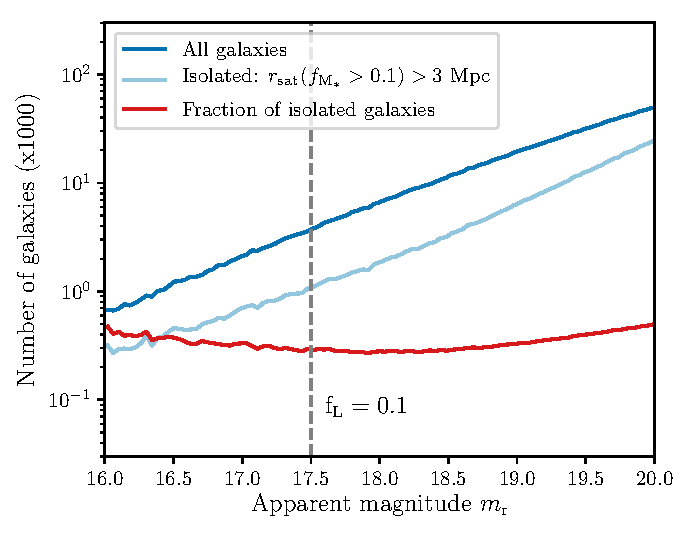
\includegraphics[width=1.0\columnwidth]{Figures/isolation_test_kids_perc0p1-3Mpc.pdf}
	\caption{The number of isolated galaxies (light blue) compared to the total number of galaxies (dark blue), as a function of apparent $r$-band magnitude $m\un{r}$. The fraction of `isolated galaxies' (red) slightly increases with apparent magnitude, because satellites fainter than the flux limit are not detected, which can cause lenses close to the magnitude limit ($m\un{lim}=20 \magn$) to be falsely identified as isolated. The dashed vertical line represents the magnitude $m\un{bright}$, below which all satellites with a luminosity fraction larger than $f\un{L} \equiv L\un{sat}/L\un{lens}=0.1$ compared to the lens are still detected.}
	\label{fig:isolation_test_fraction}
\end{figure}

\begin{figure}
	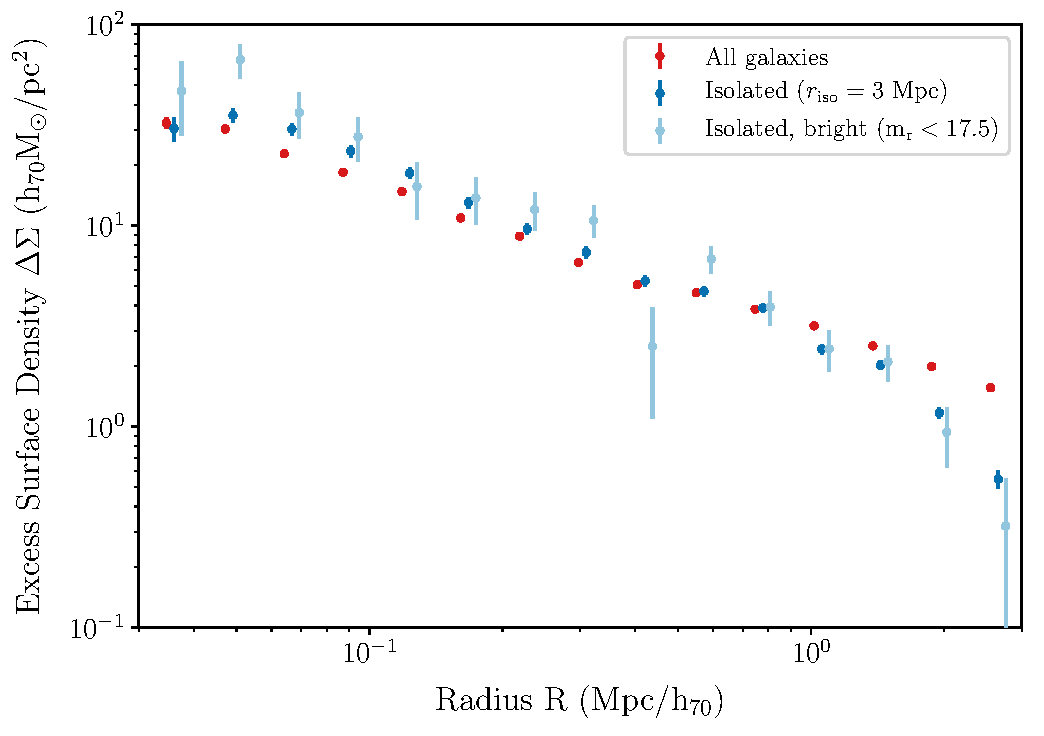
\includegraphics[width=1.0\columnwidth]{Figures/ESD_KiDS_isotest.pdf}
	\caption{To assess the effect of the magnitude limit ($m\un{lim}=20 \magn$) on the isolation criterion, we compare the ESD profile of the isolated galaxies (dark blue) with that of a more reliable `bright' sample (dark blue, $m\un{lim}<17.5 \magn$), which allows us to see all satellites down to luminosity fraction $f\un{L} \equiv L\un{sat}/L\un{lens}=0.1$. Due to the smaller number of lenses, the ESD profile of the bright isolated sample shows much larger error bars and scatter. Nevertheless, its behaviour on both small and large scales is consistent with the ESD profile of the full isolated sample, indicating that the effect the magnitude limit is limited.}
	\label{fig:isolation_test_ESD}
\end{figure}

\begin{figure}
	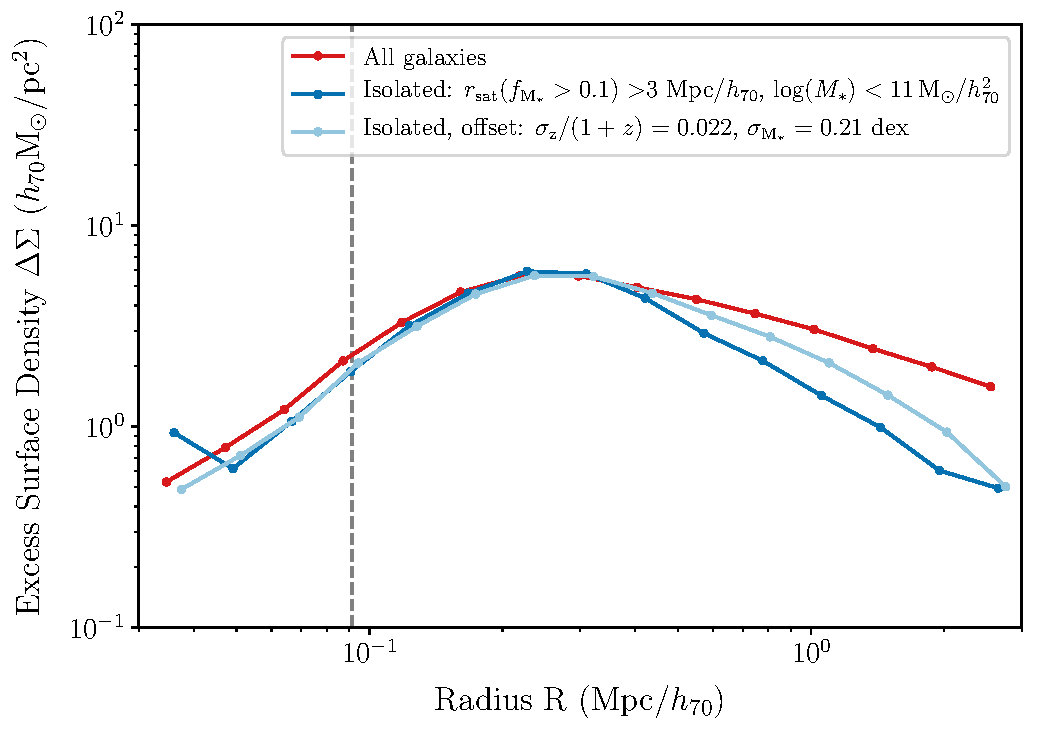
\includegraphics[width=1.0\columnwidth]{Figures/ESD_MICE_isotest_offset.pdf}
	\caption{The ESD profile of the `offset' isolated sample of MICE galaxies (light blue) selected using lenses with randomly offset redshifts ($\sigma\un{z}/(1+z) = 0.018$) and stellar masses ($\sigma\un{M_*} = 0.21$ dex). Compared to the ESD profile of the truly isolated MICE sample (dark blue) the `offset' sample has a $\sim30\%$ higher signal at large scales ($R > 0.5 \hMpc$), although it is still significantly lower than that of all MICE galaxies (red).}
	\label{fig:isolation_test_offset}
\end{figure}


\section{Conversion to the RAR}
\label{sec:conversion}

After measuring the lensing profile around a galaxy sample, the next important step is to convert it into the corresponding RAR. We start from the ESD $\Delta\Sigma(R)$ as a function of projected radius $R$ and the measured stellar masses of the lens galaxies $M\un{*}$, and aim to arrive at their observed radial acceleration $g\un{obs}$ as a function of their expected baryonic radial acceleration $g\un{bar}$. The latter can be calculated using Newton's law of universal gravitation:
\begin{equation}\label{eq:grav}
g(r) = \frac{G \, M(<r)}{r^2} \, .
\end{equation}
which defines the radial acceleration $g$ in terms of the gravitational constant $G$ and the enclosed mass $M(<r)$ within spherical radius $r$. The calculation of  $g\un{bar}$ requires the enclosed baryonic mass $M\un{bar}(<r)$ of the galaxies, which consist of both stars and gas. We discuss our construction of $M\un{bar}(<r)$ in Sect. \ref{sec:baryonic_mass}.

The calculation of $g\un{obs}$ requires the enclosed observed mass $M\un{obs}(<r)$ of the galaxy sample, which we obtain through the conversion of our observed ESD profile \mbox{$\Delta\Sigma(R)$}. To make sure this conversion is robust, we compare two different methods: a simple analytical method which assumes that DM haloes can be roughly approximated with a Singular Isothermal Sphere density model (Sect. \ref{sec:SIS_approximation}), and an elaborate numerical approach which fits a piece-wise power law to the stacked ESD profile (Sect. \ref{sec:piece-wise_powerlaw}) without any assumption on the averaged halo shape except for spherical symmetry. We validate both methods using mock surface density maps from the BAHAMAS simulation (Sect. \ref{sec:conversion_test}).

\subsection{Baryonic mass of the galaxies}
\label{sec:baryonic_mass}


The calculation of the expected baryonic radial acceleration $g\un{bar}$ requires the enclosed mass $M(<r)$ within a spherical radius $r$ around the galaxy centre. The enclosed mass of an isolated galaxy can be roughly subdivided into stars and gas, where the latter can be further distinguished into cold and hot gas.

The stellar masses of our GAMA and GL-KiDS galaxies are estimated using their multi-band spectral energy distributions, by fitting them with stellar population synthesis models (see Sect. \ref{sec:gama} and \ref{sec:gamalike_kids}). The MICE stellar masses are determined from their luminosities using $M/L$ ratios, and the BAHAMAS stellar masses from ... (see Sect. \ref{sec:mice_mocks} and \ref{sec:bahamas_mocks}). From these $M_*$ values, the fraction of cold gas $f\un{cold} = M\un{cold}/M_*$ can be estimated using scaling relations based on HI and CO observations. Following \cite{brouwer2016} we use the the best-fit scaling relation found by \cite{boselli2014}, based on the  Herschel Reference Survey \cite[]{boselli2010}:
\begin{equation}\label{eq:fcold}
	\log(f\un{cold}) = -0.69 \, \log(M_*) + 6.63 \, .
\end{equation}
We apply this equation to all observed and simulated values of $M_*$ in order to arrive at the total galaxy mass: $M\un{g} = M_* + M\un{cold} = M_* (1 + f\un{cold})$. The spatial distribution of the stellar and cold gas mass are similar \cite[]{pohlen2010,crocker2011,cooper2012,davis2013} and can therefore be considered a single mass distribution, especially for the purposes of GGL which only measures the ESD profile at scales larger than the galaxy itself ($R>30\hkpc$). Fig. \ref{fig:missing-baryons} shows the enclosed mass profiles (upper panel) and RAR (lower panel) for different baryonic components in the BAHAMAS simulation. The stellar mass at $30 \hMpc$ (red star) gives a good approximation of $M_*$ across all radii (dotted red line). We therefore model the baryonic mass of our galaxies as a point mass $M\un{g}$, containing both the stellar and cold gas mass.

However, the total baryonic mass distribution $M\un{bar}$ including hot gas can extend to much larger distances. This is shown in blue in Fig. \ref{fig:missing-baryons}, where the upper limit is given by the BAHAMAS simulation (dark blue line) and the lower limit by ... observations from \cite{tumlinson2017} (bottom of the light blue band). The region in between these lines (light blue band) represents the so-called `missing baryons' \cite[]{fukugita1998,fukugita2004,shull2012}, which are currently thought to reside in the difficult to observe Warm-Hot Intergalactic Medium \cite[WHIM,][]{nicastro2018}. This missing mass is predicted by Big Bang Nucleosynthesis \cite[BBN,][]{kirkman2003} and CMB measurements \cite[]{spergel2003,planck2014}, but can not normally be observed by multi-wavelength surveys. Our analysis can therefore not constrain the contribution to $g\un{bar}$ based on this component, although a hard upper limit at sufficiently large radii is given by the cosmic baryon fraction $f\un{b} = \Omega\un{b}/\Omega\un{m} = 0.17$ \cite[]{hinshaw2013}, which is shown in yellow. Given this inherent inability, we will the galaxy mass $M\un{g}$ as our best estimate of the total baryonic mass. We note, however, that even if the stellar+cold gas mass is not a good approximation of the total baryonic mass within $3 \hMpc$, this will not affect the comparison between our GGL observations and the different DM simulations and MG models, as long as all these predictions are based only on the mass $M\un{g}$ of the galaxy (which is the case in this work).

Concerning predictions within the $\lcdm$ framework, omitting the use of hot gas will not affect our models since the total mass distribution at the considered scales ($>30\hkpc$) is dominated by DM. Within a MG framework such as EG and MOND, where the excess gravity emanates from the baryonic matter, it is slightly more complicated. In Sect. 2.2 of \cite{brouwer2016} we carefully modelled the distribution of all baryonic components, based on observations from both GAMA and literature, including their effect on the excess gravity. We found that, for galaxies with $M_*<1\E{11}\hmsun$, the contribution to the ESD profile from hot gas and satellites was small compared to that of the stars and cold gas. Although this analysis was done for the EG theory, the effect of these extended mass distributions within MOND are similar or even less. This allows us to use a point mass $M\un{g}$ as a reasonable approximation for the baryonic mass distribution within our measurement range when computing the predictions of EG and MOND (see Sect. \ref{sec:EG} and \ref{sec:MOND}).

\begin{figure}
	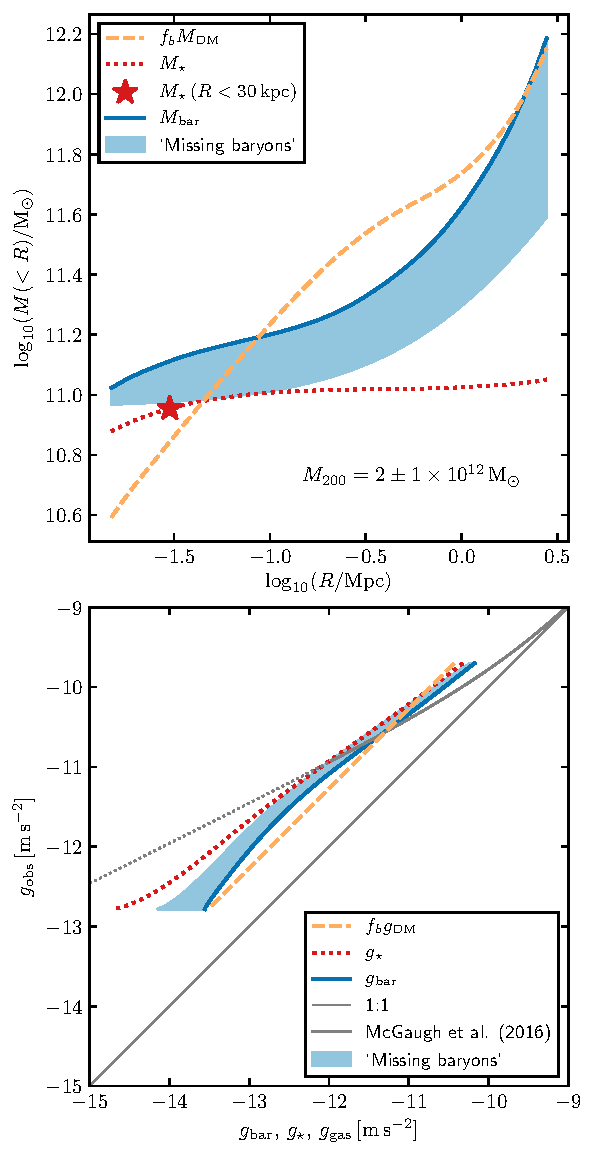
\includegraphics[width=\columnwidth]{Figures/missing_baryons.pdf}
	\caption{\emph{Upper panel: }Cumulative mass profiles of stars (dotted red) and baryons (solid blue) for BAHAMAS galaxies with $1<M_{200}/10^{12}{\rm M}_\odot<3$. The star marker indicates the stellar mass within a $30$~kpc aperture, indicative of what is typically regarded as the stellar mass of a galaxy. The blue shaded band shows an estimate based on fig.~7 of \citet{tumlinson2017} of the baryonic mass which would be `missing' in even a multi-wavelength survey. In the inner galaxy only a small fraction of the baryons are missing, but in the outer galaxy the majority are missing. The yellow dashed line shows the expected baryonic mass profile if the baryon density is everywhere equal to a fixed fraction $f_b=\Omega_b/\Omega_m$ of the local dark matter density. At large enough radii ($\gtrsim 2$~Mpc), the baryon-to-DM ratio converges to the cosmic average. \emph{Lower panel: } As in upper panel, but in acceleration space. The cosmic baryon fraction provides a robust upper limit on $g_{\rm bar}$ at low accelerations.}
	\label{fig:missing-baryons}
\end{figure}


\subsection{Singular Isothermal Sphere approximation}
\label{sec:SIS_approximation}

When calculating $g\un{obs}$ we start out from our ESD profile measurement, which consists of the value $\Delta\Sigma(R)$ measured in a set of $R$-bins. At our measurement radii ($R>30 \hkpc$) the ESD is dominated by the DM halo. We can therefore adopt the simple assumption that our observed density profile $\rho\un{obs}(r)$ is roughly described by a Singular Isothermal Sphere (SIS) model:
\begin{equation}\label{eq:rho_SIS}
	\rho\un{SIS}(r) = \frac{\sigma^2}{2 G \pi r^2} \, . 
\end{equation}
The SIS is generally considered to be the simplest parametrization of the spatial distribution of matter in an astronomical system (such as galaxies, clusters, etc.). It assumes that the dominant constituent particles (in our case DM) behave as an ideal gas that is confined by their combined spherically symmetric gravitational potential, where $\sigma$ is the total velocity dispersion of the particles. Despite its simple form, the ESD derived from the SIS profile:
\begin{equation}\label{eq:ESD_SIS}
\Delta\Sigma\un{SIS}(R) = \frac{\sigma}{2 G R} \, ,
\end{equation}
is generally able to describe WL measurements around galaxies and clusters (references). The SIS profile is therefore ideally suited to model the total enclosed mass distribution of our lenses, which can then be derived as follows:
\begin{equation}\label{eq:mass_SIS}
	M\un{SIS}(<r) = 4 \pi \int_{0}^{r}\rho\un{SIS}(r') r'^2 {\rm d} r' = \frac{2\sigma^2 r}{G} \, .
\end{equation}

Now, for each measured value of $\Delta\Sigma\un{obs}$ at its projected radius $R$, we assume that the entire density profile is described by a SIS with $\sigma$ normalized such that $\Delta\Sigma\un{SIS}(R)$ goes through $\Delta\Sigma\un{obs}$. We also assume that the considered lens is flat, in order to approximate the spherical distance $r$ with the measured transverse distance $R$. Using these assumptions, we can combine Eq. \ref{eq:ESD_SIS} and \ref{eq:mass_SIS} to compute the observed enclosed mass distribution corresponding to that measurement:
\begin{equation}
	M\un{obs} = \frac{2 (2 G R \, \Delta\Sigma) r}{G} = 4 \Delta\Sigma \, r^2 \, .
\end{equation}
Through Eq. \ref{eq:grav}, this results in a very simple expression for the observed gravitational acceleration:
\begin{equation}
g\un{obs} = \frac{G (4 \Delta\Sigma \, r^2)}{r^2} = 4 G \Delta\Sigma \, ,
\end{equation}
computed at each point along the ESD profile.


\subsection{Piece-wise power law density profile}
\label{sec:piece-wise_powerlaw}

We can instead assume a more self-consistent form for the volume density profile and parametrize it as a piece-wise power law constrained to be continuous. This comes at the cost of needing to invert the non-linear function $\Delta\Sigma(\rho)$, which we achieve via an iterative method. We choose to parametrize $\rho(r)$ in terms of $N$ pairs of values $(r_n,\rho_n)$ such that the slope $a_n$ and normalization $b_n$ of the power law profile segments are:
\begin{align}
\log\rho &= a_n \log(r) + b_n \\
a_n &= \frac{\log(\rho_{n+1})-\log(\rho_n)}{\log(r_{n+1})-\log(r_n)}\\
b_n &= \log(\rho_n) - a_n\log(r_n)\\
(a_n, b_n) &=
\begin{cases}
(a_0, b_0) & {\rm if}\ r < r_0\\
(a_n, b_n) & {\rm if}\ r_n \leq r < r_{n+1}\\
(a_{N-1}, b_{N-1}) & {\rm if}\ r \geq r_N
\end{cases}
\label{eq:rho_piecewise_powerlaw}\end{align}
(Throughout, $\log$ denotes the natural logarithm.) We provide an expression for the discrete excess surface density profile in terms of the volume density profile, i.e. the function to be inverted, in Appendix~\ref{sec:appendix_invert_esd}.

In order to invert $\Delta\Sigma_m(\rho_n)$, we take as constant the values $\{R_m\}$, $\{\Delta\Sigma_m\}_{\rm obs}$ and $\{r_n\}$. We then propose an initial guess $\{\rho_n\}$ which we perturb iteratively, calculating the corresponding $\{\Delta\Sigma_m\}$ at each iteration and comparing with $\{\Delta\Sigma_m\}_{\rm obs}$ via the likelihood function:
\begin{align}
\log\mathcal{L} &\propto -\frac{1}{2}(\Delta\Sigma_{\rm obs}-\Delta\Sigma)^{\rm T}\Sigma^{-1}(\Delta\Sigma_{\rm obs}-\Delta\Sigma)
\end{align}
Note that $\Sigma$ is the covariance matrix for the $\Delta\Sigma_{\rm obs}$, not to be confused with the surface density. We use the package {\sc emcee} \citep{foreman-mackey13} to estimate the posterior probability distribution of $\{\rho_n\}$, and subsequently of the corresponding $\{g_{{\rm obs},n}\}$ via integration of the volume density profile.


\subsection{Testing the RAR conversion with BAHAMAS}
\label{sec:conversion_test}

\section{Theoretical predictions}
\label{sec:theories}

\subsection{Modified Newtonian Dynamics}
\label{sec:MOND}

With his theory of Modified Newtonian Dynamics (MOND), \cite{milgrom1983} postulated that the `missing mass problem' in galaxies is not caused by an undiscovered fundamental particle, but that instead our current gravitational theory should be revised. MOND's basic premise is that one can adjust Newtons second law of motion ($F=ma$) by inserting a general function $\mu(a/a_0)$, which only comes into play when the acceleration $a$ of a test mass $m$ is much smaller than a critical acceleration $a_0$. The goal of this function is to facilitate the discovered flat rotation curves in the outskirts of galaxies, while still reproducing the Newtonian behaviour of the inner disk. In short, the force $F$ becomes:
\begin{align}\label{eq:mond_f}
	& F(a) = m \, \mu(\frac{a}{a_0}) \, a \, ,
	& \mu(x \gg 1) \approx 1 \, , \, \mu(x \ll 1) \approx x \, .
\end{align}
This implies that $a\gg a_0$ represents the Newtonian regime where $F\un{N} = m \, a\un{N}$ as expected, while $a\gg a_0$ represents the `deep-MOND' regime where $F\un{dm}=m \, a\un{dM}^2/a_0$. In a circular orbit, this is reflected in the deep-MOND gravitational acceleration $g\un{dM} \equiv a\un{dM}$ as follows:
\begin{align}\label{eq:mond_g}
	& F\un{dM} = m \frac{a\un{dM}^2}{a_0} = \frac{G \, M m}{r^2}
	& \rightarrow \,  g\un{dM} = \sqrt{a_0 \frac{G M}{r^2}} \, .
\end{align}
This can be written in terms of the expected baryonic acceleration $g\un{bar}=GM/r^2$ as follows:
\begin{equation}
	g\un{dM}(g\un{bar}) = \sqrt{a_0 \, g\un{bar}} \, ,
\end{equation}
which demonstrates that MOND predicts a very simple relation for the RAR: $g\un{obs}=g\un{bar}$ in the Newtonian regime ($g\un{obs}\gg a_0$), and following Eq. \ref{eq:mond_g} in the deep-MOND regime ($g\un{obs}\ll a_0$). However, since $\mu(a/a_0)$ (also known as the `interpolating function') is not specified by \cite{milgrom1983}, there is no specific constraint on the behaviour of this relation in between the two regimes. In the work of \cite{milgrom2008}, several families of interpolation functions are discussed. Selecting the third family (given by their Eq. 13) with constant parameter $\alpha=1/2$, provides the function that M16 later used to fit to their measurement of the RAR using rotation curves 153 galaxies. This relation can be written as:
\begin{equation}\label{eq:mcgaugh}
	g\un{obs} = \frac{g\un{bar}}{1 - e^{-\sqrt{g\un{bar}/a_0}}} \, .
\end{equation}
where $a_0 \equiv g\un{\dagger}$ corresponds to the fitting parameter constrained by M16 to be $g\un{\dagger}=1.20\pm26\E{-10} {\rm m/s^2}$. Since Eq. \ref{eq:mcgaugh} (equal to Eq. 4 in M16) is also considered a viable version of the MOND interpolation function by \cite{milgrom2008}, we will consider it the baseline prediction of MOND in this work. As the baseline value of $a_0$, we will likewise use the value of $g\un{\dagger}$ measured by M16, since it exactly corresponds to the value of $a_0=1.2\E{-10} {\rm m/s^2}$ considered canonical in MOND since it's first measurement by \cite{begeman1991}, using the rotation curves of 10 galaxies.

\subsection{Emergent Gravity}
\label{sec:EG}

The work of \cite{verlinde2016} (V16 hereafter), which is embedded in the framework of string theory and holography, shares the view that the missing mass problem is to be solved through a revision of our current gravitational theory. Building on the ideas of \cite{jacobson1995,jacobson2016,padmanabhan2010,faulkner2015} and his own previous work \cite[]{verlinde2011}, V16 abandons the notion of gravity as a fundamental force. Instead, it emerges from an underlying microscopic description of space-time, in which the notion of gravity has no a-priori meaning.

The aforementioned earlier works have shown that constructing a theory EG in a static (`anti-de Sitter') universe allows for the re-derivation Einstein's laws of GR. A distinguishing feature of V16 is that it attempts to describe an expanding (`de Sitter') universe, which is filled with a DE component. This results in a new volume law for gravitational entropy caused by DE, in addition to the area law normally used to retrieve Einsteinian gravity. According to V16, energy that is concentrated in the form of a baryonic mass distribution causes an elastic response in the entropy of the surrounding DE. This results in an additional gravitational component at scales set by the `Hubble acceleration scale' $a\un{0} = c H_0$. Here $c$ is the speed of light, and $H_0$ is the current Hubble constant which measures the Universe's expansion velocity.

Because this extra gravitational component is predicted to explain the effects usually attributed to DM, it is often expressed as an \emph{apparent} dark matter (ADM) distribution:
\begin{equation}
M_{\rm D}^2 (r) = \frac{  cH_0 r^2}{6G} \frac{d\left( M_{\rm b}(r) r \right)}{dr} \, .
\label{eq:veg_mdm}
\end{equation}
Thus the ADM distribution is completely defined by the baryonic mass distribution $M\un{b}(r)$ as a function of the spherical radius $r$, and a set of known physical constants.

Since we measure the ESD profiles of galaxies at projected radial distances $R>30 \hsMpc$, we can assume that their baryonic component is enclosed within the minimal measurement radius \cite[see also][]{brouwer2017}. This is equivalent to describing the galaxy as a point mass $M\un{b}$, which allows us to simplify Eq. \ref{eq:veg_mdm} to:
\begin{equation}
M_{\rm D}(r)=\sqrt{\frac{cH_{0} \, M_{\rm b}}{6 \, G}} \, r \, .
\end{equation}
Now the total enclosed mass, $M\un{EG}(r) = M\un{b} + M\un{D}(r)$, can be used to calculate the predicted gravitational acceleration $g\un{EG}(r)$ as follows:
\begin{equation}
	g_{\rm EG}(r) = \frac{G M\un{EG}(r)}{r^2} = \frac{G M\un{b}}{r^2} + \sqrt{\frac{cH_{0}}{6}} \, \frac{\sqrt{G M_{\rm b}}}{r} \, .
\end{equation}
In terms of the expected baryonic acceleration $g\un{bar}(r) = G M\un{b}/r^2$, this simplifies even further to:
\begin{equation}
g_{\rm EG}(g\un{bar}) = g\un{bar} + \sqrt{\frac{cH_{0}}{6}} \, \sqrt{g\un{bar}} \, .
\end{equation}

Note that Eq. \ref{eq:veg_mdm} is only a macroscopic approximation of the underlying microscopic phenomena described at the start of this section, and is thus only valid for static, spherically symmetric and isolated baryonic mass distributions. For this reason, we select only the most isolated galaxies from our sample (see Sect. \ref{sec:isolation}), such that our WL measurements are not influenced by neighbouring galaxies. In addition, cosmological evolution of the $H_0$ parameter is not yet implemented in the theory, restricting its validity to galaxies with relatively low redshifts. However, we calculate that at our mean lens redshift ($\langle z \rangle \sim 0.2$) using an evolving $H(z)$ would result in only a $~5\%$ difference in our ESD measurements, based on the background cosmology used in this work.

In order to test V16 using the standard WL methodology, we need to assume that the deflection of photons by a gravitational potential in this alternative theory corresponds to that in GR. This assumption is justified because, in EG's original (anti-de Sitter) form, Einstein's laws emerge from its underlying description of space-time. The additional gravitational force described by ADM does not affect this underlying theory, which is an effective description of GR. Therefore, we assume that the gravitational potential of an ADM distribution produces the same lensing shear as an equivalent distribution of actual matter.

\subsection{Analytical CDM model}
\label{sec:analytical}

To help guide an intuitive interpretation of the lensing RAR within the framework of the $\Lambda$CDM theory, we make use of the simple model of N17 which combines a basic model of galactic structure and scaling relations to predict the RAR. We refer to N17 for a full description, but give a summary here. A galaxy of a given stellar (or baryonic -- there is no distinction in this model)  mass occupies a dark matter halo of a mass fixed by the abundance matching relation of \citet{Behroozi13}. The dark halo concentration is fixed to the cosmological mean for haloes of that mass \citep{Ludlow14}. The baryonic disc follows an exponential surface density profile with a half-mass size fixed to $0.2\times$ the scale radius of the dark halo (N17). The above is sufficient to specify the cumulative mass profile of both the baryonic and dark components of the model galaxy; calculating $g_{\rm obs}$ and $g_{\rm bar}$ is then straightforward.

\section{Results}
\label{sec:results}
Write when the results are ready.

\subsection{Isolated galaxies}

Plot: GAMA + MICE + BAHAMAS \\
Plot: KiDS + MICE + BAHAMAS

\subsection{Galaxies in 4 stellar mass bins}

Plot: KiDS + MICE

\subsection{Isolated galaxies in 4 stellar mass bins}

Plot: KiDS + MICE + BAHAMAS

\begin{figure}
	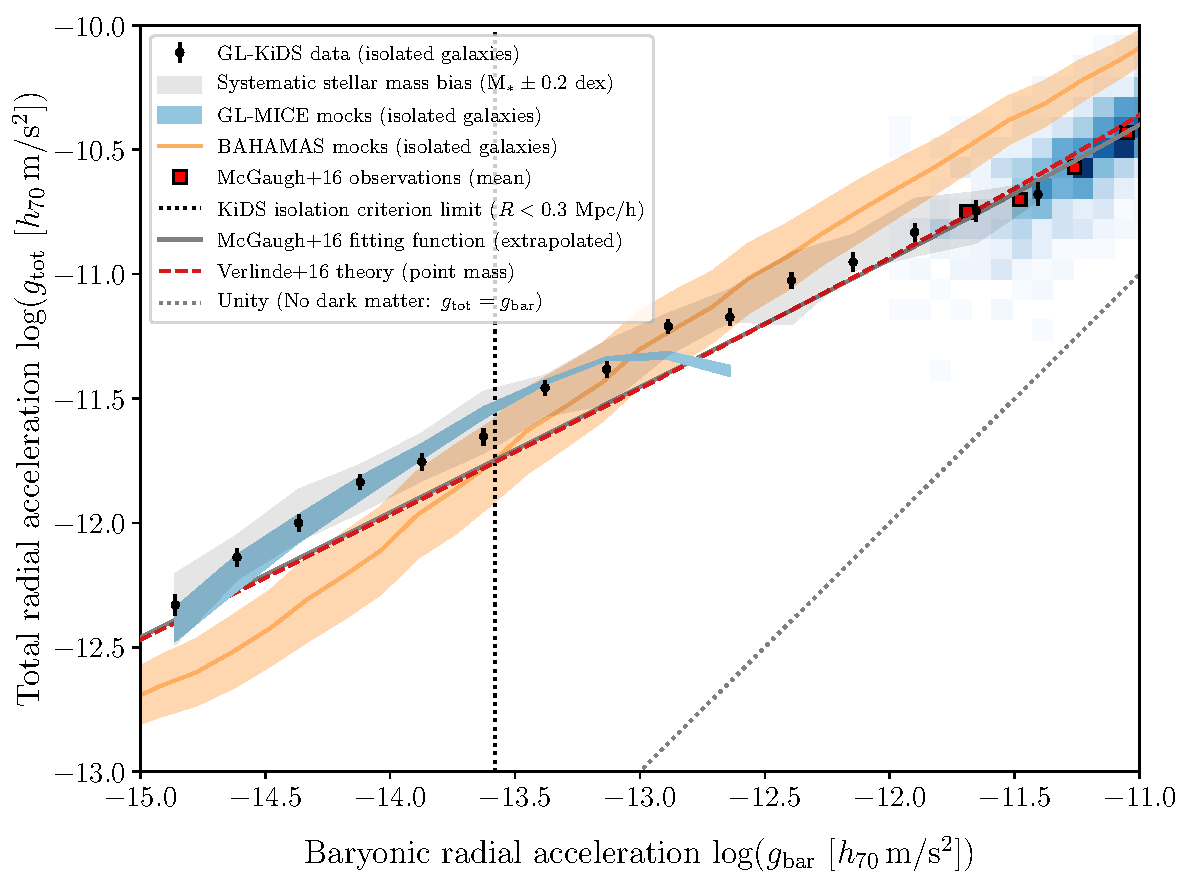
\includegraphics[width=1.0\columnwidth]{Figures/RAR_KiDS+MICE+Bahamas_No_Nobins_isolated.pdf}
	\caption{TBW}
	%\label{fig:}
\end{figure}

\subsection{Stellar mass bins}

\begin{figure*}
	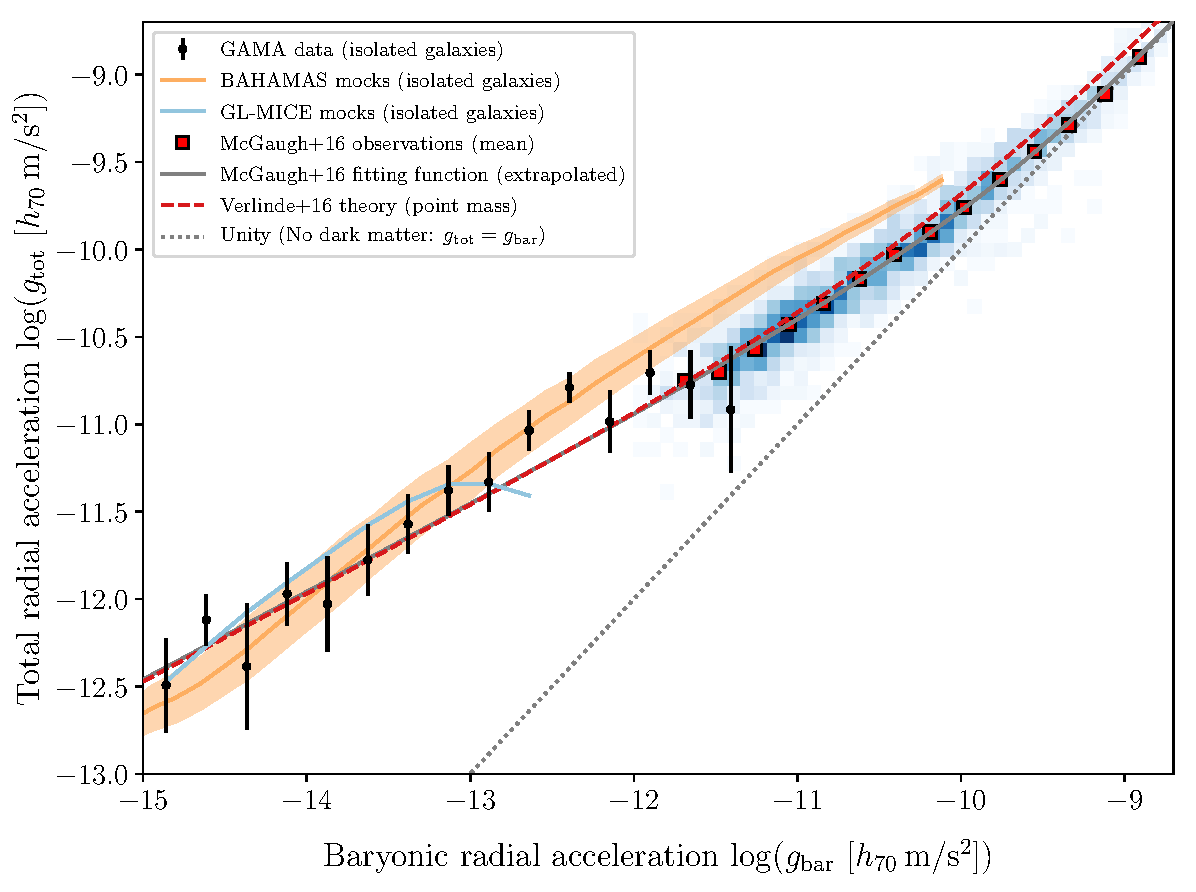
\includegraphics[width=1.0\textwidth]{Figures/RAR_GAMA+MICE+Bahamas_Nobins_isolated_zoomout.pdf}
	\caption{TBW}
	%\label{fig:}
\end{figure*}

\begin{comment}

\begin{figure*}
	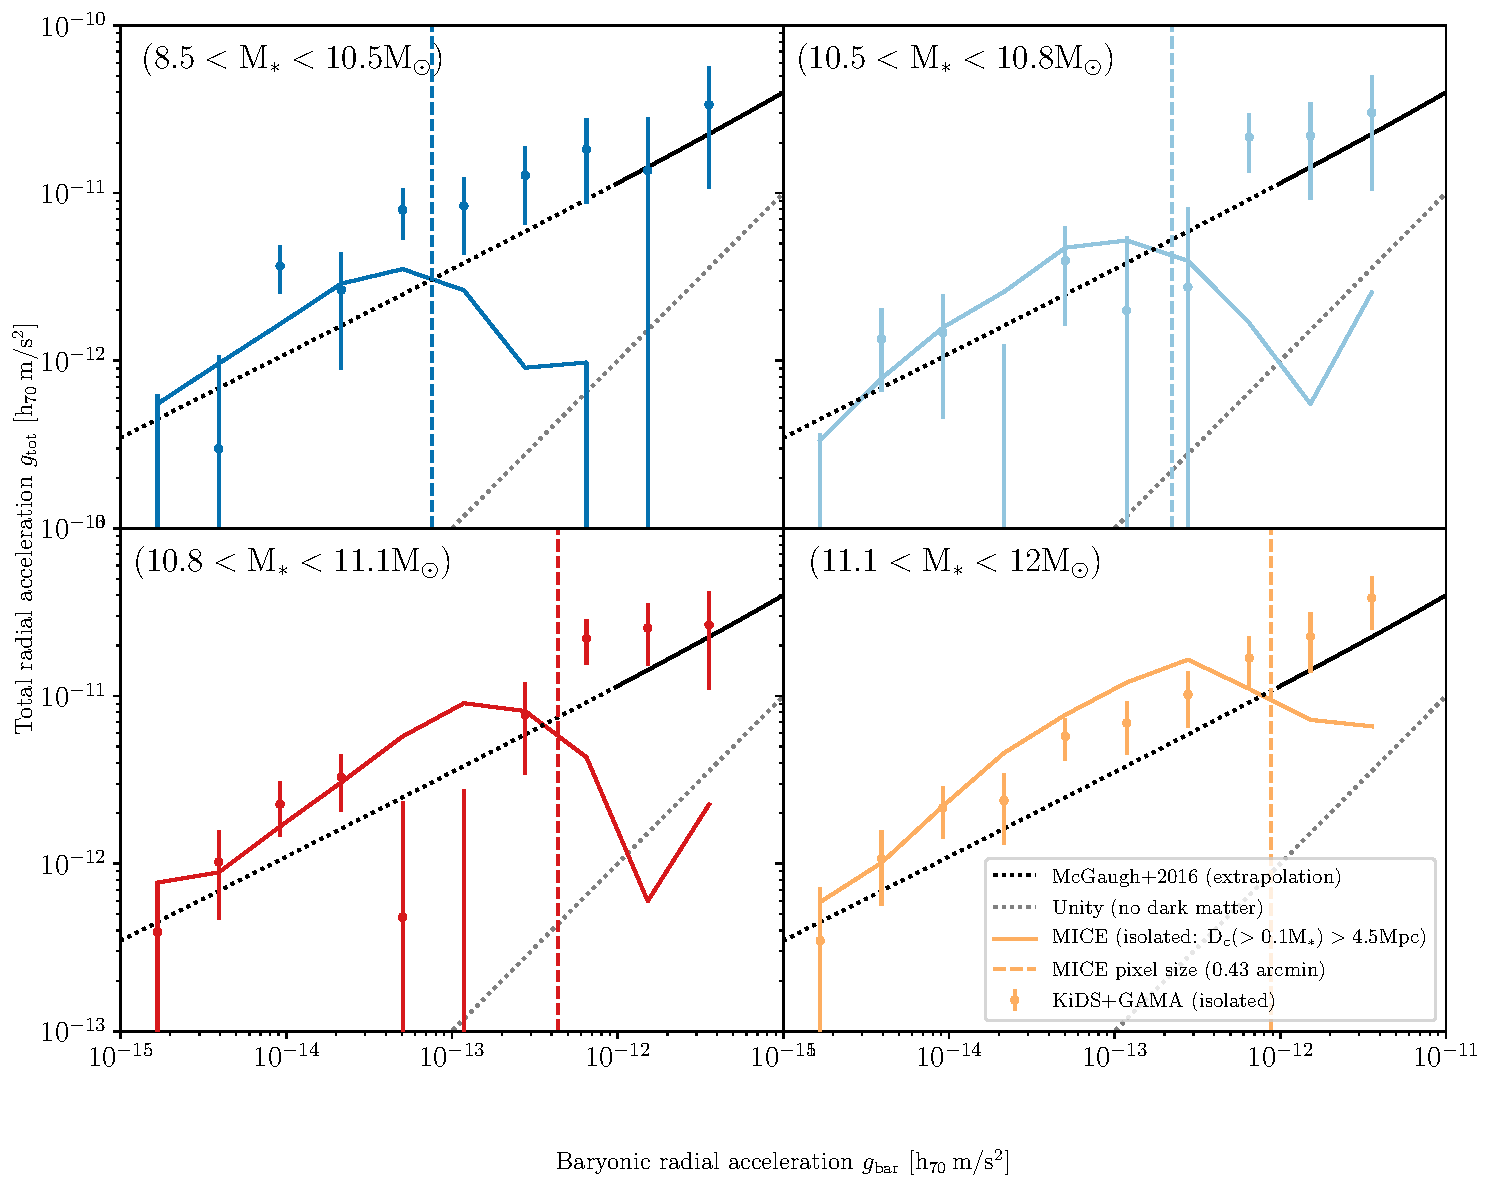
\includegraphics[width=1.0\textwidth]{Figures/RAR_GAMA+MICE_4-massbins_isolated_strong.pdf}
	\caption{TBW}
	%\label{fig:}
\end{figure*}

\begin{figure*}
	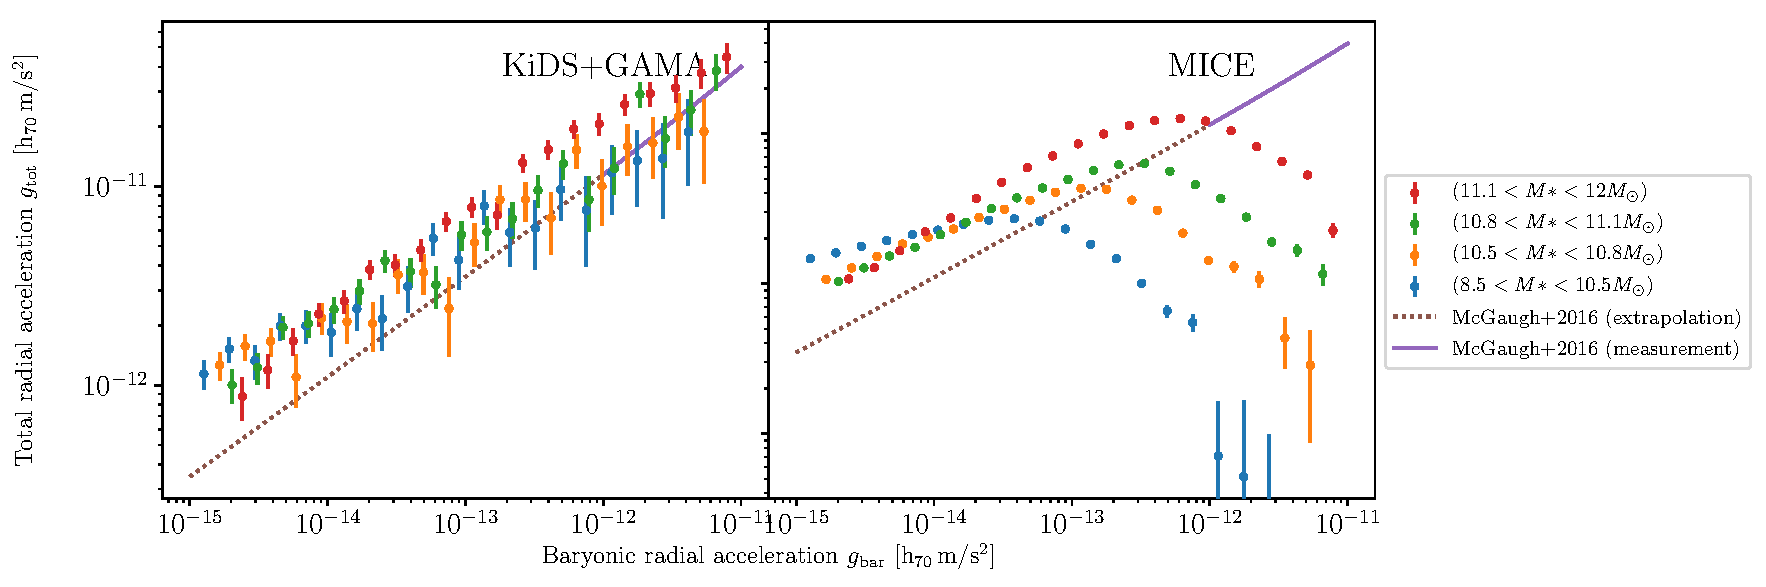
\includegraphics[width=1.0\textwidth]{Figures/RAR_KiDS+MICE_massbins-8p5_10p5_10p8_11p1_12p0_transverse.pdf}
	\caption{TBW}
	%\label{fig:}
\end{figure*}

\end{comment}


\section{Discussion and conclusion}
\label{sec:discon}

\section*{Acknowledgements}
Write at the end.

\begin{comment}
KAO acknowledges support from VICI grant 016.130.338 of the Netherlands Foundation for Scientific Research (NWO).

We are indebted to Ian McCarthy, who provided the BAHAMAS data products used in our analysis.

We are grateful to \url{https://math.stackexchange.com} user Paul Enta for providing an expression for one of the integrals needed in Appendix~\ref{sec:appendix_invert_esd}.

This work is partly based on tools and data products produced by GAZPAR operated by CeSAM-LAM and IAP.

V. Demchenko acknowledges the Higgs Centre Nimmo Scholarship and the Edinburgh Global Research Scholarship. J. Harnois-D{\'e}raps is supported by the European Commission under a Marie-Sk{\l}odowska-Curie European Fellowship (EU project 656869). M. Bilicki is supported by the Netherlands Organization for Scientific Research, NWO, through grant number 614.001.451. C. Heymans acknowledges support from the European Research Council under grant number 647112. H. Hoekstra acknowledges support from Vici grant 639.043.512, financed by the Netherlands Organization for Scientific Research. K. Kuijken acknowledges support by the Alexander von Humboldt Foundation. H. Hildebrandt is supported by an Emmy Noether grant (No. Hi 1495/2-1) of the Deutsche Forschungsgemeinschaft. P. Schneider is supported by the Deutsche Forschungsgemeinschaft in the framework of the TR33 `The Dark Universe'. E. van Uitert acknowledges support from an STFC Ernest Rutherford Research Grant, grant reference ST/L00285X/1.

Computations for the $N$-body simulations were performed in part on the Orcinus supercomputer at the WestGrid HPC consortium (\url{www.westgrid.ca}), in part on the GPC supercomputer at the SciNet HPC Consortium. SciNet is funded by: the Canada Foundation for Innovation under the auspices of Compute Canada; the Government of Ontario; Ontario Research Fund - Research Excellence; and the University of Toronto.

This research is based on data products from observations made with ESO Telescopes at the La Silla Paranal Observatory under programme IDs 177.A-3016, 177.A-3017 and 177.A-3018, and on data products produced by Target OmegaCEN, INAF-OACN, INAF-OAPD and the KiDS production team,  on behalf of the KiDS consortium. OmegaCEN and the KiDS production team acknowledge support by NOVA and NWO-M grants. Members of INAF-OAPD and INAF-OACN also acknowledge the support from the Department of Physics \& Astronomy of the University of Padova, and of the Department of Physics of Univ. Federico II (Naples).

GAMA is a joint European-Australasian project based around a spectroscopic campaign using the Anglo-Australian Telescope. The GAMA input catalogue is based on data taken from the Sloan Digital Sky Survey and the UKIRT Infrared Deep Sky Survey. Complementary imaging of the GAMA regions is being obtained by a number of independent survey programs including GALEX MIS, VST KiDS, VISTA VIKING, WISE, Herschel-ATLAS, GMRT and ASKAP providing UV to radio coverage. GAMA is funded by the STFC (UK), the ARC (Australia), the AAO, and the participating institutions. The GAMA website is \url{www.gama-survey.org}.

This work has made use of CosmoHub \cite[]{carretero2017}. CosmoHub has been developed by the Port d'Informaci{\'o}n Cient{\'i}fica (PIC), maintained through a collaboration of the Institut de F{\'i}sica d'Altes Energies (IFAE) and the Centro de Investigaciones Energ{\'e}ticas, Medioambientales y Tecnol{\'o}gicas (CIEMAT), and was partially funded by the ``Plan Estatal de Investigaci{\'o}n Cient{\'i}fica y T{\'e}cnica y de Innovaci{\'o}n'' program of the Spanish government.

This work has made use of {\scshape python} (\url{www.python.org}), including the packages {\scshape numpy} (\url{www.numpy.org}) and {\scshape scipy} (\url{www.scipy.org}). Plots have been produced with {\scshape matplotlib} \cite[]{hunter2007matplotlib}. The mock shear profiles from MICE are computed using {\scshape TreeCorr} (\url{https://pypi.python.org/pypi/TreeCorr}).

\emph{Author contributions:} All authors contributed to the development and writing of this paper. The authorship list is given in three groups: the lead authors (M. Brouwer, V. Demchenko, J. Harnois-D{\'e}raps), followed by two alphabetical groups. The first alphabetical group includes those who are key contributors to both the scientific analysis and the data products. The second group covers those who have either made a significant contribution to the data products, or to the scientific analysis.
end{comment}
\end{comment}
%%%%%%%%%%%%%%%%%%%%%%%%%%%%%%%%%%%%%%%%%%%%%%%%%%

%%%%%%%%%%%%%%%%%%%% REFERENCES %%%%%%%%%%%%%%%%%%

% The best way to enter references is to use BibTeX:

\bibliographystyle{mnras}
\bibliography{biblio}


%%%%%%%%%%%%%%%%%%%%%%%%%%%%%%%%%%%%%%%%%%%%%%%%%%

%%%%%%%%%%%%%%%%%%%%%%%%%%%%%%%%%%%%%%%%%%%%%%%%%%

\appendix
\onecolumn
\section{Excess surface density profile of a piece-wise power law volume density profile}
\label{sec:appendix_invert_esd}

\noindent The excess surface density profile is measured in a series of discrete radial bins with edges $R_m$. The representative value at the centre of the bin -- here we define the bin centre as $\frac{1}{2}(R_m+R_{m+1})$, i.e. not the `logarithmic centre' $\sqrt{R_mR_{m+1}}$, which ensures accuracy in the calculation of the mean enclosed surface density -- is $\Delta\Sigma_m=\overline{\Sigma}_m-\Sigma_m$, where $\overline{\Sigma}_m$ is the mean surface density within $\frac{1}{2}(R_m+R_{m+1})$ and $\Sigma_m$ is the surface density averaged over the interval $[R_m,R_{m+1})$. We give an expression for this discrete excess surface density profile in terms of the parametric form for $\rho(r)$ given in Eq.~\ref{eq:rho_piecewise_powerlaw}.

The mean enclosed surface density is:
\begin{align}
  \overline{\Sigma}_m &= \frac{1}{\pi R_mR_{m+1}}\left[I_1(0, \sqrt{R_0R_1}, \tilde{a}_0, \tilde{b}_0) + 
\sum_{k=0}^m I_1(\sqrt{R_mR_{m+1}},\sqrt{R_{m+1}R_{m+2}}, \tilde{a}_m, \tilde{b}_m)\right]\\
  \tilde{a}_m &= \frac{\log(\Sigma_{m+1})-\log(\Sigma_m)}{\frac{1}{2}\left(\log(R_{m+2})-\log(R_m)\right)}\\
  \tilde{b}_m &= \log(\Sigma_m) - \frac{1}{2}\tilde{a}_m\log(R_mR_{m+1})\\
  I_1(R_i,R_j,\tilde{a},\tilde{b}) &= \frac{2\pi e^{\tilde{b}}}{\tilde{a}+2}\left(R_j^{a+2} - R_i^{a+2}\right)
\end{align}
\noindent and the local surface density is given by:
\begin{align}
  \Sigma_m &= \sum_{n=0}^{N-1}
  \begin{cases}
    0 & {\rm if}\ r_{n+1} < R_m\\
    \frac{4e^{b_n}}{R_{m+1}^2-R_m^2} \left(-I_2(r_{n+1},R_m,a_n)\right) & {\rm if}\ r_n < R_m\ {\rm and}\ R_m \leq r_{n+1} < R_{m+1}\\
    \frac{4e^{b_n}}{R_{m+1}^2-R_m^2} \left(I_2(r_{n+1},R_{m+1},a_n)-I_2(r_{n+1},R_m,a_n)\right) & {\rm if}\ r_n < R_m\ {\rm and}\ r_{n+1} \geq R_{m+1}\\
    \frac{4e^{b_n}}{R_{m+1}^2-R_m^2} (I_2(r_{n+1},r_n,a_n)-I_2(r_{n+1},R_m,a_n)\\ \quad +I_2(r_n,R_m,a_n)+I_2(r_{n+1},R_{m+1},a_n)\\ \quad -I_2(r_{n+1},r_n,a_n)) & {\rm if}\ R_m \leq r_n < R_{m+1}\ {\rm and}\ r_n \geq R_{m+1}\\
    \frac{4e^{b_n}}{R_{m+1}^2-R_m^2} (I_2(r_{n+1},R_{m+1},a_n)-I_2(r_{n+1},R_m,a_n)\\ \quad -I_2(r_n,R_{m+1},a_n)+I_2(r_n,R_m,a_n)) & {\rm if}\ r_n \geq R_{m+1}\\
    \frac{4e^{b_n}}{R_{m+1}^2-R_m^2} (I_2(r_{n+1},r_n,a_n)-I_2(r_{n+1},R_m,a_n)\\ \quad +I_2(r_n,R_m,a_n)-I_2(r_{n+1},r_n,a_n)) & {\rm if}\ r_n \geq R_m\ {\rm and}\ r_{n+1} < R_m\\
  \end{cases}\\
  I_2(r,R,a) &=
  \begin{cases}
    -\frac{1}{3}R^{a+3}\left(\frac{r^2}{R^2}-1\right)^{\frac{3}{2}}{}_2{\rm F}_1\left(\frac{3}{2},-\frac{a}{2};\frac{5}{2};1-\frac{r^2}{R^2}\right) & {\rm if}\ r\ {\rm is}\ {\rm finite}\\
    \frac{\sqrt{\pi}}{2}\frac{\Gamma\left(-\frac{a+1}{2}\right)}{\Gamma\left(-\frac{a}{2}\right)}\frac{R^{a+3}}{a+3} & {\rm if}\ r=\infty
  \end{cases}
\end{align}
where ${}_2{\rm F}_1(\cdot,\cdot;\cdot;\cdot)$ is the Gaussian hypergeometric function and $\Gamma(\cdot)$ is the Gamma function.

% Don't change these lines
\bsp	% typesetting comment
\label{lastpage}
\end{document}

% End of mnras_template.tex
